\documentclass[review]{elsarticle}
\usepackage{comment}
\usepackage{url}
\usepackage[breaklinks]{hyperref}
\usepackage{breakurl}
\usepackage[ruled]{algorithm2e}

\journal{Optics \& Laser Technology}

\bibliographystyle{elsarticle-num}

\usepackage{graphicx}
\usepackage{subcaption}
\usepackage[svgnames]{xcolor}
\usepackage{amsmath}
\usepackage{amsfonts}
\usepackage{amssymb}
 
\begin{document} 

\begin{frontmatter}

\title{Illumination Dependency in Dynamic Laser Speckle Analysis}

\author{Fernando Pujaico Rivera}
\author{Roberto Alves Braga, Jr.}

\address{Federal University of Lavras, Lavras, Brazil}
\fntext[myfootnote2]{201518201@posgrad.ufla.br}
\fntext[myfootnote1]{robertobraga@deg.ufla.br }

\begin{abstract}
We analyse how the frequency bands 
influence the independence 
of speckle index values from the level of illumination
%of the value speckle index from the level of illumination 
in a dynamic laser speckle analysis.
Specifically, 
we study how the temporal speckle deviation 
index is influenced by the use of three different frequency bands of the speckle signal.
Finally, it is shown how signals with high frequency components return values with greater independence of the level of illumination.
\end{abstract}

\begin{keyword}
Biospeckle laser \sep 
Biospeckle index \sep 
Biospeckle signal\sep 
Biological activity \sep
Dynamic speckle 
\end{keyword}

\end{frontmatter}

\linenumbers

\section{Introduction}
Dynamic laser speckle is a phenomenon that is used to monitor changes in laser illuminated samples. It can be measured by several different indices \cite{BSLTLBOOK}. These indices are associated to the level of changes and can be expressed by numerical and or graphical outcomes that can be affected by filtering during the image processing \cite{RIVERA2017144}. As an example, we have  the AVD \cite{avd} and 
IM \cite{ARIZAGA1999163} indices, that filter
the information present in the history of the speckle images like a first-order high pass filter with a cut-off in the middle
of the normalized frequency band.
For this reason, it is important to analyse how
the chosen frequency band alters the result of a selected index.
On the other hand, there is still a limitation in making a speckle analysis in the presence of inhomogeneous illumination, because
most biospeckle indices are influenced
by the use of a specific level of illumination \cite{REIS2016}.
The level of illumination can vary regarding the profile of the sample, such as an apple \cite{KAZ:12a} or the very irregular surface present in a kefir \cite{kefir}.
It can also vary in accordance with the moisture present in a seed \cite{CARDOSO2011} due to the penetration of the light in the sample, or even when the colour of the sample varies, such as in the interface between cancerous and normal tissues \cite{BCB+:12a}.
This is the reason why there has been a continual search for an adequate index, despite the fact there are many indices presented in the literature \cite{BSLTLBOOK}, but still without a solution that is independent of the intensity of the illumination.
The move toward portable equipment \cite{Bra:17} reinforces the need to search for such methods and their relation with the illumination.
Thus, the present work aims to establish a relation between the frequency band used
and the speckle index; particularly in the dependence of
the temporal speckle deviation matrix \cite{Nothdurft:05} on the level of illumination.


\section{Description of the system}
\label{sec:description}

\subsection{Data for ink drying test}
\label{sec:descriptionink}
Fig.~\ref{fig:system} shows the system setup of the ink sample test during drying, where
a red laser was pointed at a layer of ink drying, monitored by a digital camera;
the images were collected receiving two different illumination levels, 
because the neutral density lens partially covers the laser beam \cite{REIS2016}.
The images were turned into data-sets:
the data was acquired with a sampling rate of $F_s=$ 12.5 hertz, with 
$N=400$ images collected per data-set. In all, there were collected $11$ data-sets 
(each one with the two different illumination levels) at minutes 
$0$, $10$, $20$, $30$, $40$, $50$, $60$, $75$, $105$, $120$ and $150$ of the drying process.
\begin{figure}[ht!]
\centering
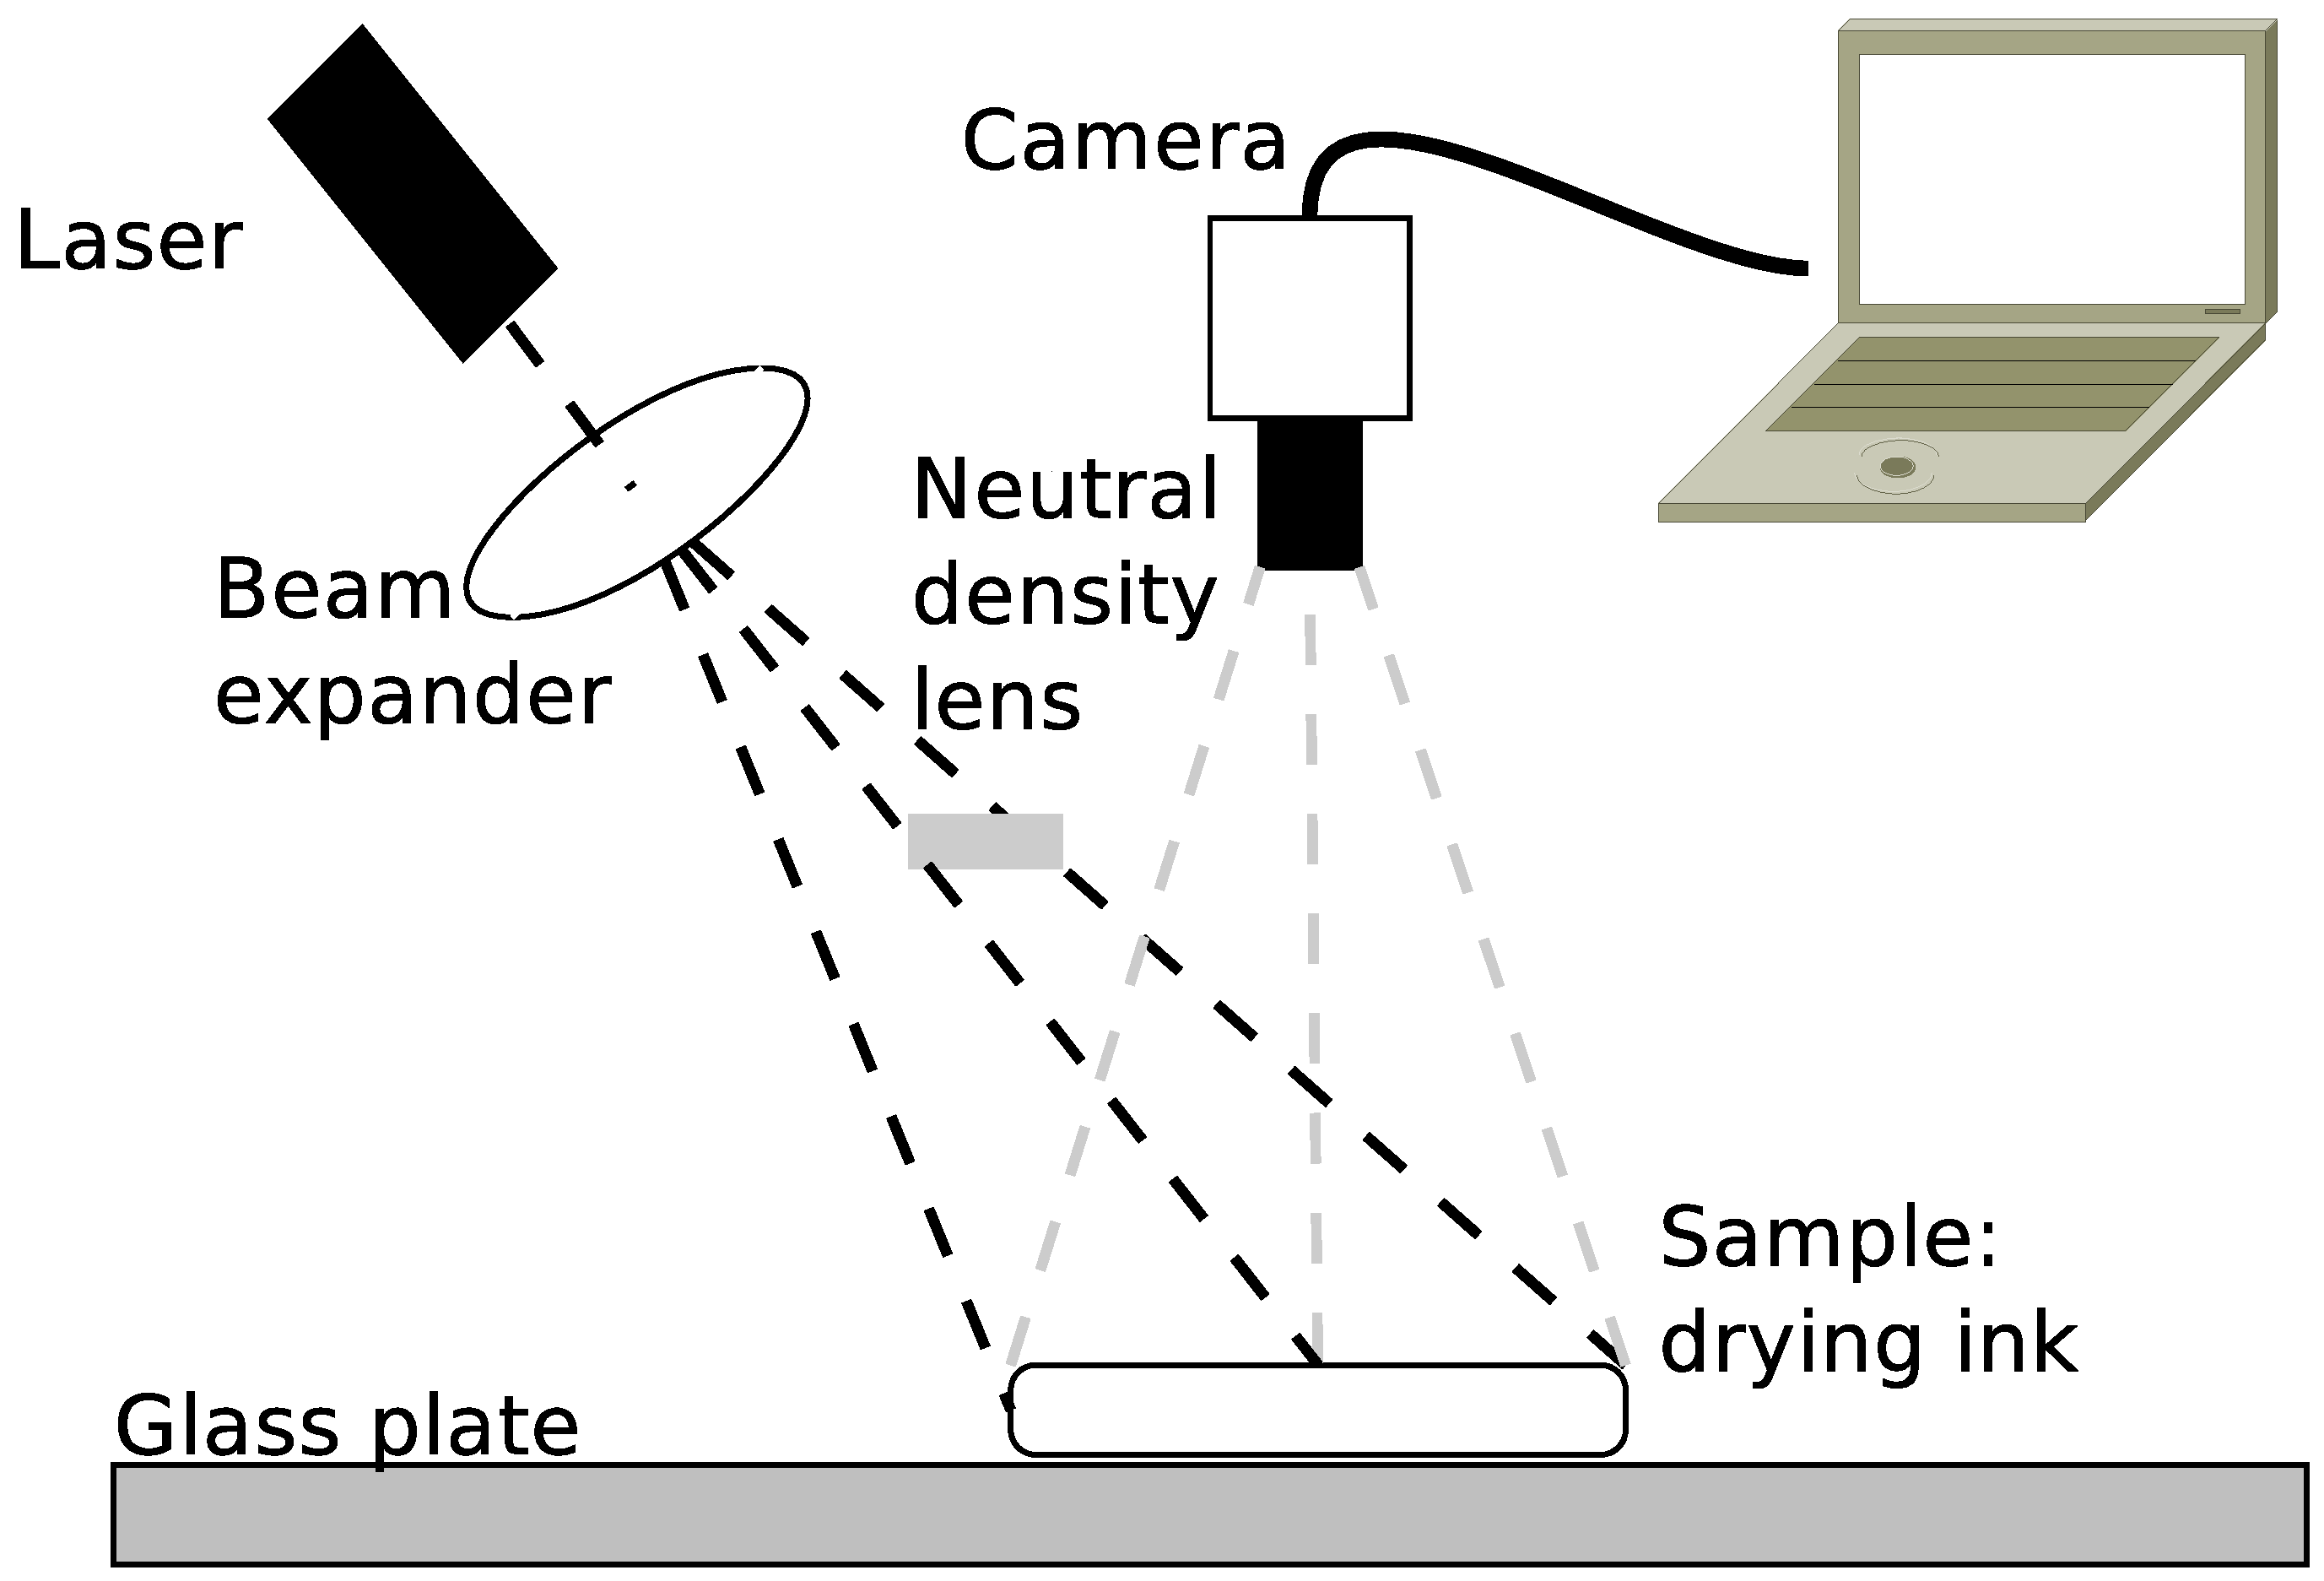
\includegraphics[width=0.65\columnwidth]{system.eps}
\caption{Experimental configuration of dynamic laser speckle formation monitored by digital system 
with the levels of illumination over a layer of ink drying.}
\label{fig:system}
\end{figure}
Two $250\times200$-pixel regions were selected from each image of the data-sets, 
corresponding to regions with two different levels of illumination, 
as shown with red lines in Fig.~\ref{fig:regions}; thus, 
in the right side of Fig.~\ref{fig:regions}  we have the
portion of image that was altered by the neutral density lens,
 so that this side has low illumination, and
the left side has a high illumination.
\begin{figure}[h!]
\centering
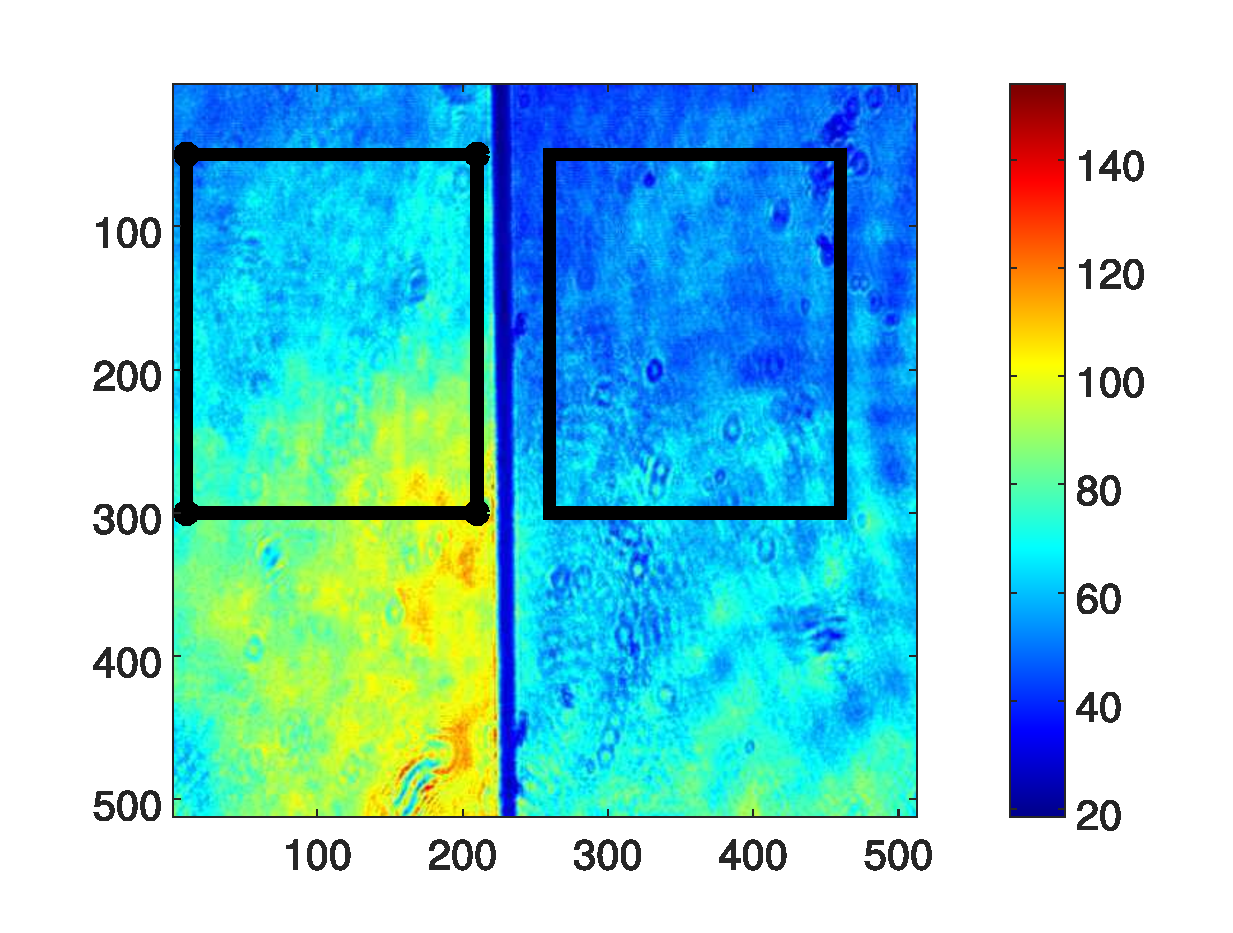
\includegraphics[width=0.85\columnwidth]{meanall_points_all.eps}
\caption{Selected regions and light intensity distribution in the ink drying test.}
\label{fig:regions}
\end{figure}

\subsection{Data for steady state paper test}
\label{sec:descriptionpaper}
The test over steady state paper has a similar configuration, as seen in
Fig.~\ref{fig:system} with the absence of 
the neutral density lens.
The phenomenon observed was the variation of the speckle signal associated with  the speckle response of the material, 
the experimental setup of the camera, the resolution of the images and also to the mechanical noise; 
so that one data-set was collected sampled with a frequency of $F_s=$ 10 hertz. 
In all, there were $N=129$ 640$\times$480-pixel images collected.
Fig.~\ref{fig:meanpaper} represents
with a colour bar the result of calculating the temporal speckle mean matrix ($\mu$) using Eq.~(\ref{eq:cont1})
of Section~\ref{subsec:deviation}; thus, it is easy to see how the
laser illumination in piece of paper
%level of illumination by the laser of the paper 
has an elliptical form, being highest 
close to the top of the image.
\begin{figure}[h!]
\centering
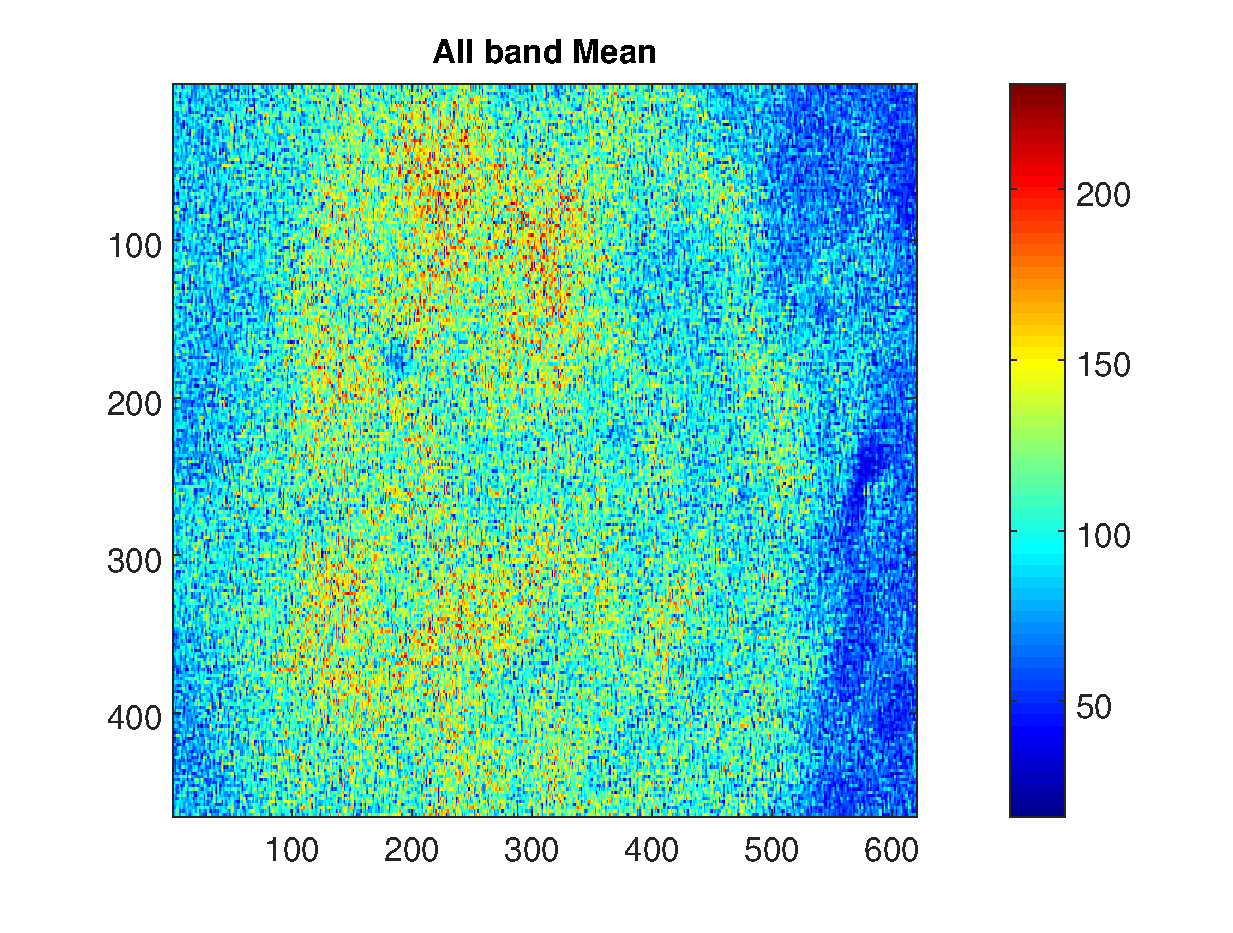
\includegraphics[width=0.85\columnwidth]{meanall.eps}
\caption{Light intensity distribution in the paper test piece with highest illumination 
presented by red pixels and lowest by blue pixels.}
\label{fig:meanpaper}
\end{figure}

\section{Numerical analysis}
\label{sec:analysis}

The sampling frequency used in the analysis of each test 
was selected so as to achieve the best speed of sampling to observe 
an appropriate frequency band of each phenomenon.
The purpose of these two tests is to observe the behaviour of the indices in two cases: 
one with an homogeneous activity level in space and time, and another with a heterogeneous activity level.
Thus, given that the paper activity test and the ink drying test are independent events, 
without comparison between them, their sampling frequencies are different,
and selected according to the best behaviour of the curves, 
higher sampling frequencies being more appropriate for the ink drying test.

\subsection{Data filtering in three frequency bands}
\label{subsec:firfilters}
Each data-set or sub-set ($P_T$) went through a filter bank with 4 outputs. Each
one had a different type of processing. The first one was trivial: 
the data was passed through without change. This data-set is referred to as $P_T$. The other three outcomes
return  signals filtered in different frequency bands: 
the band between $[0,\frac{1}{3}]\frac{F_s}{2}$ (low frequencies),
the band between $[\frac{1}{3},\frac{2}{3}]\frac{F_s}{2}$ (intermediate frequencies) and
the band between $[\frac{2}{3},1]\frac{F_s}{2}$ (high frequencies). This ultimately yields the data-sets 
$P_X$, $P_Y$ and $P_Z$, respectively; as can be seen in Fig.~\ref{fig:firfilters}.
The filtered data of the images were made using cascades
of two low-pass Finite Impulse Response (FIR) filters of order $32$, so that
$P_X+P_Y+P_Z=P_T$.
\begin{figure}[h!]
\centering
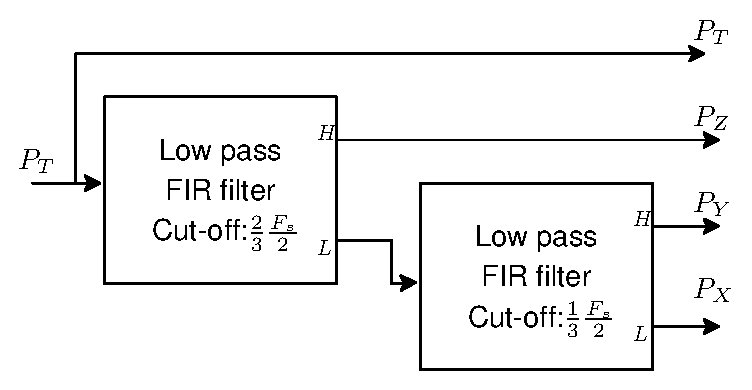
\includegraphics[width=0.55\columnwidth]{firfilters.eps}
\caption{Filtering the data-sets.}
\label{fig:firfilters}
\end{figure}

\subsection{Temporal speckle deviation matrix}
\label{subsec:deviation}
The temporal speckle deviation matrix ($\sigma$) \cite{Nothdurft:05},
used to compare the results, was obtained from the $N$ images of the data-set $P$.
We designate each image matrix in $P$ as $\mathbf{I}_{k}$, $1\leq k \leq N$, 
with $k$ an integer that indicates whether the $k$-th image $\mathbf{I}_{k}$ in the data-set was used.
Thus, the following equation was used to get
the matrix $\sigma$:
\begin{equation}\label{eq:cont2}
\sigma  = \sqrt{ \frac{1}{N} \sum_{k=1}^{N} (\mathbf{I}_{k}-\mu)^2  },
\end{equation}
so that the matrix $\mu$ can be calculated as
\begin{equation}\label{eq:cont1}
\mu =  \frac{1}{N} \sum_{k=1}^{N} \mathbf{I}_{k}.
\end{equation}
In these last two equations, all the operations are matricial, 
so that each element (i.e.\ pixel) $\mathbf{I}_{k}(i)$ in the matrix $\mathbf{I}_{k}$
should be processed with its  counterpart $\mathbf{I}_{k+1}(i)$ in the matrix $\mathbf{I}_{k+1}$.


Aditionally, the temporal speckle deviation index can be defined as $\bar{\sigma}=<\sigma>$, the mean value
of all elements in the matrix $\sigma$, with $<.>$ being the mean spatial operator.


\subsection{Fujii matrix}
\label{subsec:fujii}

The Fujii matrix \cite{Fujii:87} is obtained from the $N$ images in $P$.
Similarly to Section~\ref{subsec:deviation}, 
we designate each image matrix in $P$ as $\mathbf{I}_{k}$, $1\leq k \leq N$.
Thus, the following equation is used to get the Fujii matrix:
\begin{equation}\label{eq:contFujii2}
Fujii  = \frac{1}{N-1} \sum_{k=1}^{N-1} \frac{|\mathbf{I}_{k}-\mathbf{I}_{k+1}|}{\mathbf{I}_{k}+\mathbf{I}_{k+1}}.
\end{equation} 
The mean value of the Fujii matrix can be defined as $\overline{Fujii}=<Fujii>$, the mean value
of all elements in the $Fujii$ matrix.

The Fujii method is an attempt to eliminate 
the dependence of a speckle index on the level 
of illumination. For this purpose, the method defines the index as the mean value of the  first-order high pass FIR filter 
$\mathbf{I}_{k}-\mathbf{I}_{k+1}$, similarly to the  AVD index \cite{avd};
but in the Fujii method the values are corrected using an approximation of the mean value of the intensity, 
$\frac{\mathbf{I}_{k}+\mathbf{I}_{k+1}}{2}$.
This aspect of the calculation is the strong point of the method,
because the method assumes that the increase in the dynamic range of the speckle 
light ($\mathbf{I}_{k}-\mathbf{I}_{k+1}$) 
will be linear in proportion with the increase in the laser light ($\frac{\mathbf{I}_{k}+\mathbf{I}_{k+1}}{2}$).
This means that the method already uses the high frequency components
of the speckle signal, 
and discards those of low frequency, 
in addition to attempting to correct or  normalize the values of the index.
It is for these reasons that it has an acceptable performance in
eliminating or decreasing the dependence of the index on the level of intensity of the laser light.

Additionally, there is defined the matrix $Fujii_{\alpha}$, 
as the index of the filtered version of $P$ in the frequency band $\alpha$,  using the following equation:
\begin{equation}\label{eq:contFujii3}
Fujii_{\alpha}  = \frac{1}{N-1} \sum_{k=1}^{N-1} \frac{|\mathbf{(I_{\alpha})}_{k}-\mathbf{(I_{\alpha})}_{k+1}|}{\mathbf{I}_{k}+\mathbf{I}_{k+1}}.
\end{equation}
It is important to stress that the numerator of this equation 
uses the signal in the matrices $\mathbf{(I_{\alpha})}_{k}$, which are filtered versions in the frequency band $\alpha$,
of the matrix $\mathbf{I}_{k}$.
On the ohter hand, the denominator uses the signal $\mathbf{I}_{k}$, which employs the complete frequency band.
This modification was implemented because the numerator, in the calculation, 
represents or tries be the mean value of the intensity of the speckle light, 
and its value tends to zero in frequency bands without 0 hertz components.


\subsection{Data processing in the ink drying test}
\label{subsec:numprocink}

There are two levels of illumination in the ink drying regions.
For this reason, we  separated each data-set into two sub-sets
(high and low illumination), representing each one of the regions shown in Fig.~\ref{fig:regions}.
These sub-sets were filtered,
obtaining $P_T$, $P_X$, $P_Y$ and $P_Z$, which were used to obtain
\begin{figure}[h!]
\centering
\includegraphics[width=0.65\columnwidth]{filtering.eps}
\caption{Filtering of data-sets.}
\label{fig:filtering}
\end{figure}
the temporal speckle deviation matrix and the 
temporal speckle deviation indices $\bar{\sigma}_T$, $\bar{\sigma}_X$, $\bar{\sigma}_Y$ and
$\bar{\sigma}_Z$.

\subsection{Statistical analysis of relation between the matrices $\sigma$ and $\mu$}
\label{subsec:statistical}
We define $\sigma_i$ and $\mu_i$
as the values in the $i$th position in $\sigma$  
and $\mu$, respectively. We also define $\mu_p$
as the value of any element of $\mu$.
We also define the set $S_{\mu_p}=\{\sigma_i: \mu_i\equiv \mu_p; \forall i\}$
as the set of all values of $\sigma_i$  given that $\mu_i\equiv\mu_p$.
We thus obtain the vectors $L_p$, $\sigma_p$ and
$e_p$ using all the values $\mu_p$:
\begin{itemize}
 \item $L_p(\mu_p)=card\left(S_{\mu_p}\right)$,  where $L_p(\mu_p)$ is the number of elements
 in the set $S_{\mu_p}$ and $card(.)$ means the cardinality of a set.
 \item $\sigma_p(\mu_p)=mean\left(S_{\mu_p}\right)$, where $\sigma_p(\mu_p)$
 is the mean of the elements in the set $S_{\mu_p}$, with $mean(.)$ denoting the mean value operator.
 \item $e_p(\mu_p)=std\left(S_{\mu_p}\right)$, where $e_p(\mu_p)$
 is the standard  deviation of the elements in the set $S_{\mu_p}$, with $std(.)$ denoting `standard deviation'.
\end{itemize}
In practice, the vectors will only be taken using the values of $\mu_p$
with $L_p(\mu_p)>200$ samples, to establish a limit to consider a set of representative samples.


\subsection{Data processing in the steady state paper test}
\label{subsec:numprocink}

In this test we have one data-set that was filtered (\ref{fig:filtering2}) 
obtaining $P_T$, $P_X$, $P_Y$ and $P_Z$, where the outcomes are the temporal speckle mean matrix and the 
temporal speckle deviation matrix, as can be seen in Fig.~\ref{fig:filtering2}.

\begin{figure}[h!]
\centering
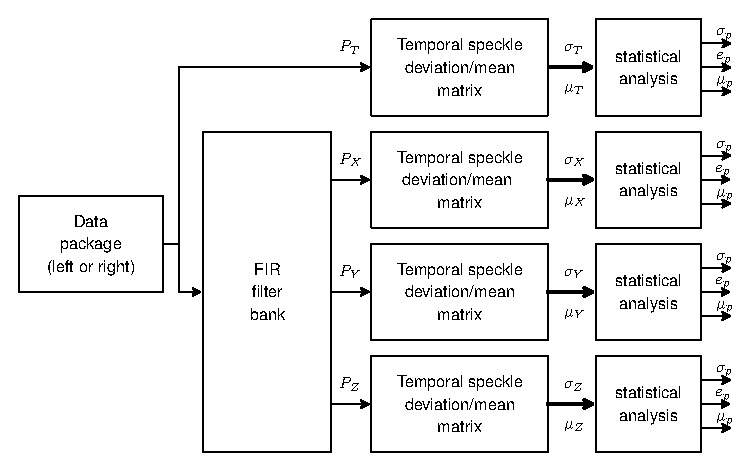
\includegraphics[width=0.65\columnwidth]{filtering2.eps}
\caption{Filtering of the steady paper data-set, obtaining the mean and the deviation.}
\label{fig:filtering2}
\end{figure}

\section{Numerical results} 
\label{sec:numerical}

In the analysis, the minimum greyscale value 
is fixed by the minimum light observable by the camera or the minimum speckle light intensity in the material analysed.
The maximum greyscale value
is fixed by the maximum light observable by the camera or the maximum speckle light intensity in the material analysed.

\subsection{Numerical results in the ink drying test} 
\label{subsec:numericalink}

The activity level analysis in the ink drying process has as objective to analyse 
the behaviour of the speckle index in a  dynamic process,
in the context of a system that changes its characteristics over time.

In Fig.~\ref{fig:numerical}, we can see the result of processing 
 the data for the ink drying test under the dynamic laser speckle index (DLSI) in two areas with 
different level of illumination. Fig.~\ref{fig:allink}
represents $\bar{\sigma}_T$ for two light intensity levels. It was obtained using $P_T$
over time, with the complete frequency bands.
Fig.~\ref{fig:stdxink}
represents $\bar{\sigma}_X$ for two light intensity levels, using $P_X$
over time, with the frequency band between $0$ and $\frac{1}{3}\frac{F_s}{2}$\ Hz.
Fig.~\ref{fig:stdyink}
represents $\bar{\sigma}_Y$ for two light intensity levels, using $P_Y$
over time, with the frequency band between $\frac{1}{3}\frac{F_s}{2}$ and $\frac{2}{3}\frac{F_s}{2}$ Hz.
Fig.~\ref{fig:stdzink}
represents $\bar{\sigma}_Z$ for two light intensity levels, using $P_Z$
over time, with the frequency band between $\frac{2}{3}\frac{F_s}{2}$ and $\frac{F_s}{2}$ Hz.
\begin{figure}[h!]
    \centering
    \begin{subfigure}[b]{0.475\textwidth}
        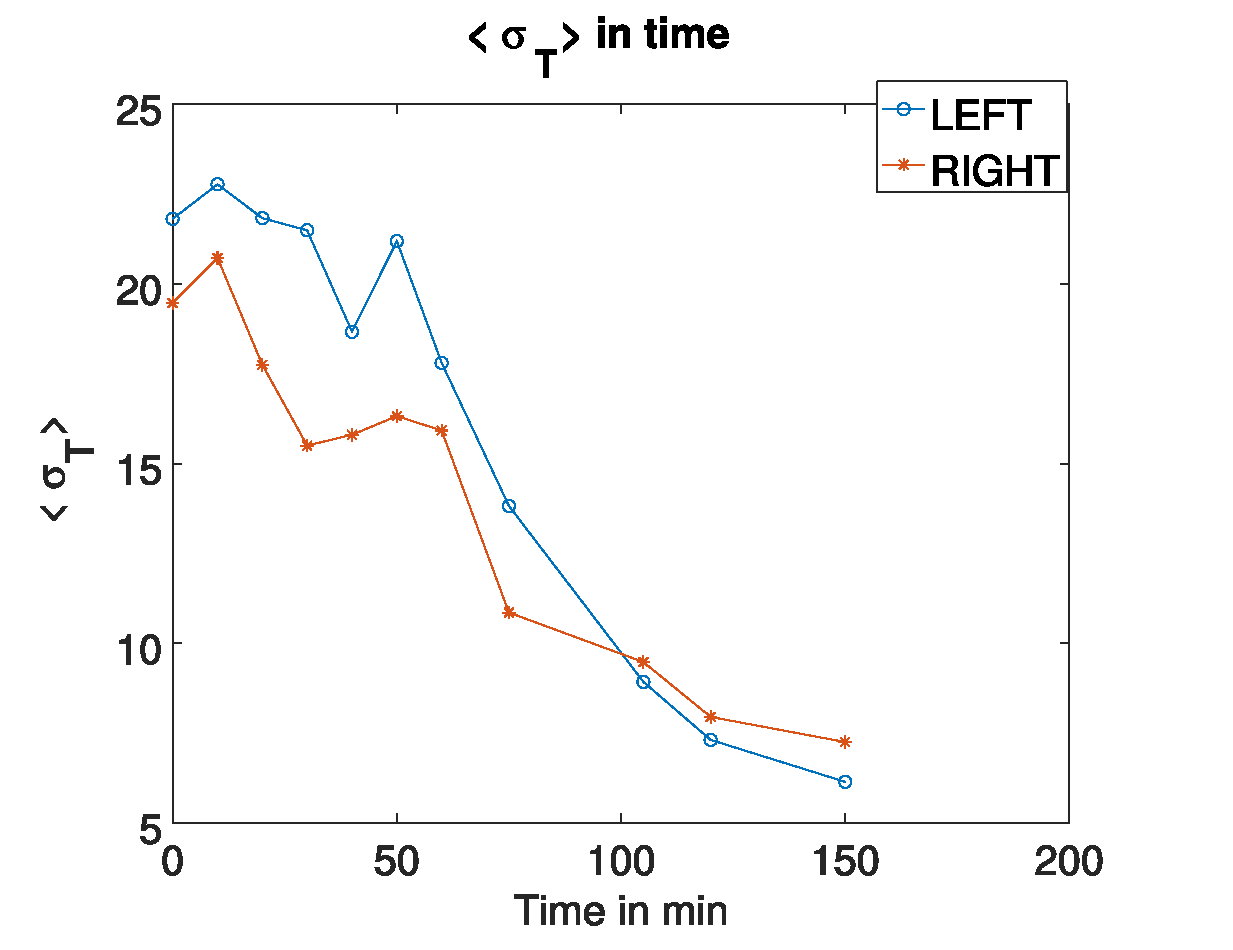
\includegraphics[width=\textwidth]{std-all.eps}
	\caption{$\bar{\sigma}_T$ over time.}
        \label{fig:allink}
    \end{subfigure}
    ~
    \begin{subfigure}[b]{0.475\textwidth}
        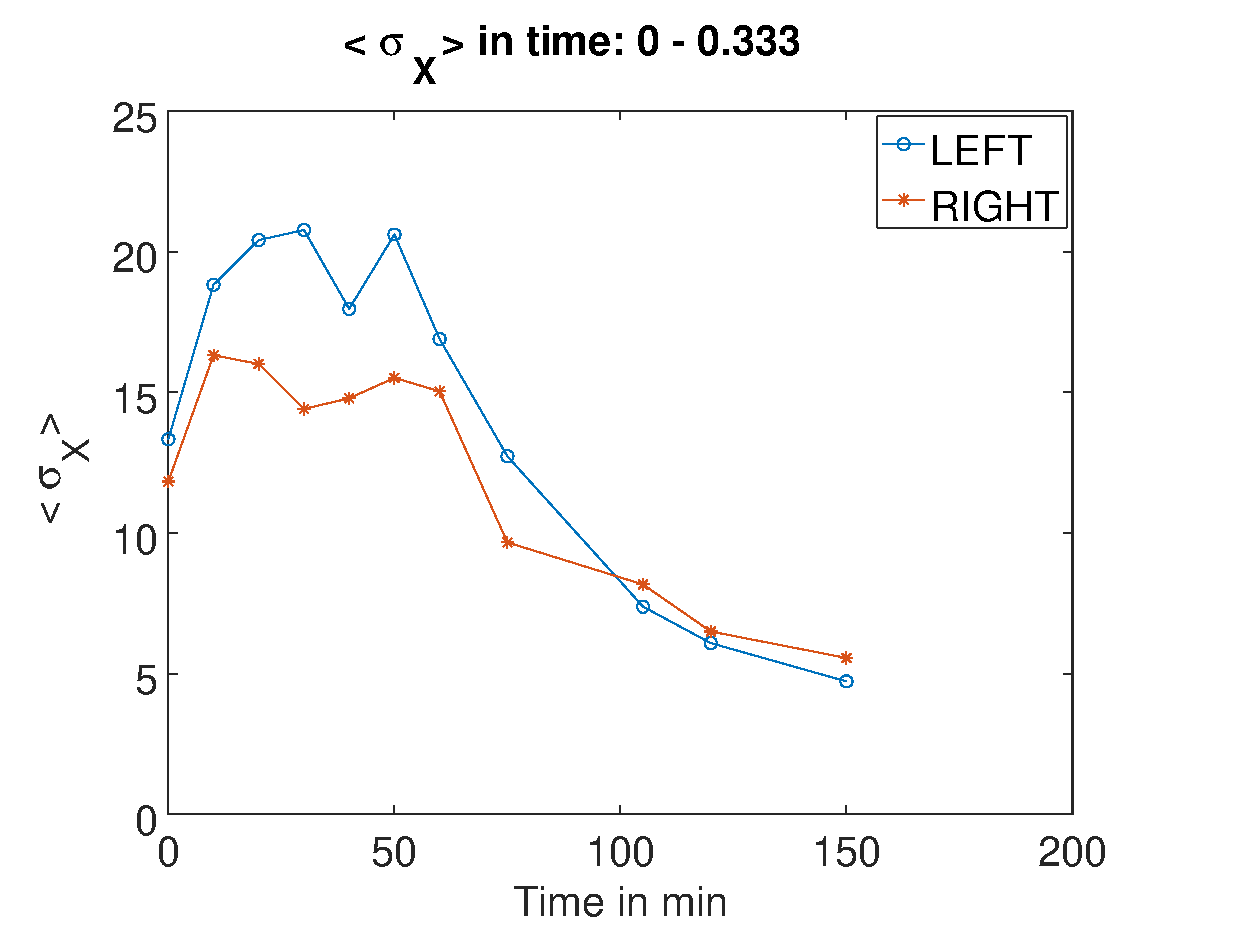
\includegraphics[width=\textwidth]{std-bandx.eps}
	\caption{$\bar{\sigma}_X$ over time.}
        \label{fig:stdxink}
    \end{subfigure}
    ~\\ 
    \begin{subfigure}[b]{0.475\textwidth}
        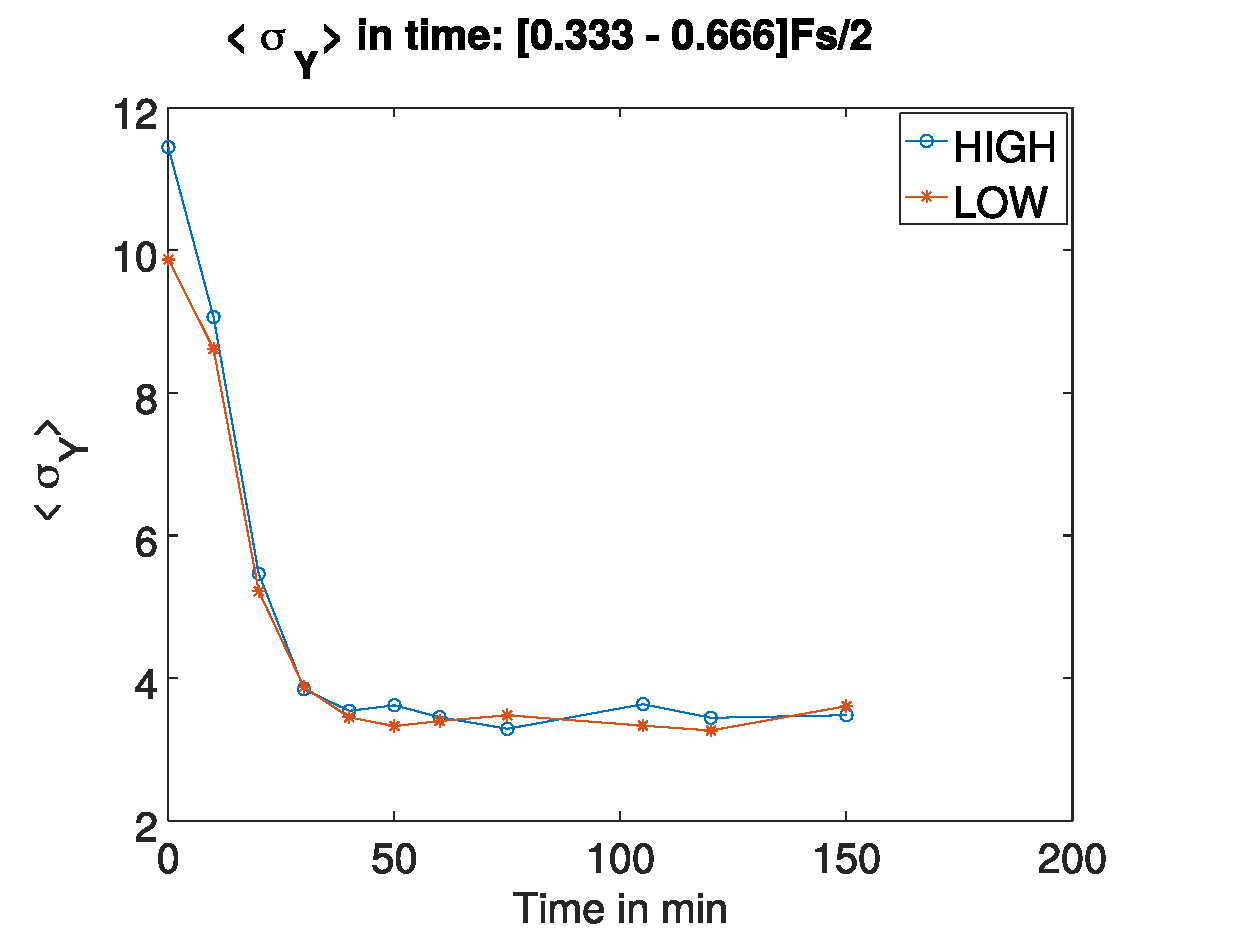
\includegraphics[width=\textwidth]{std-bandy.eps}
	\caption{$\bar{\sigma}_Y$ over time.}
        \label{fig:stdyink}
    \end{subfigure}
  ~
    \begin{subfigure}[b]{0.475\textwidth}
        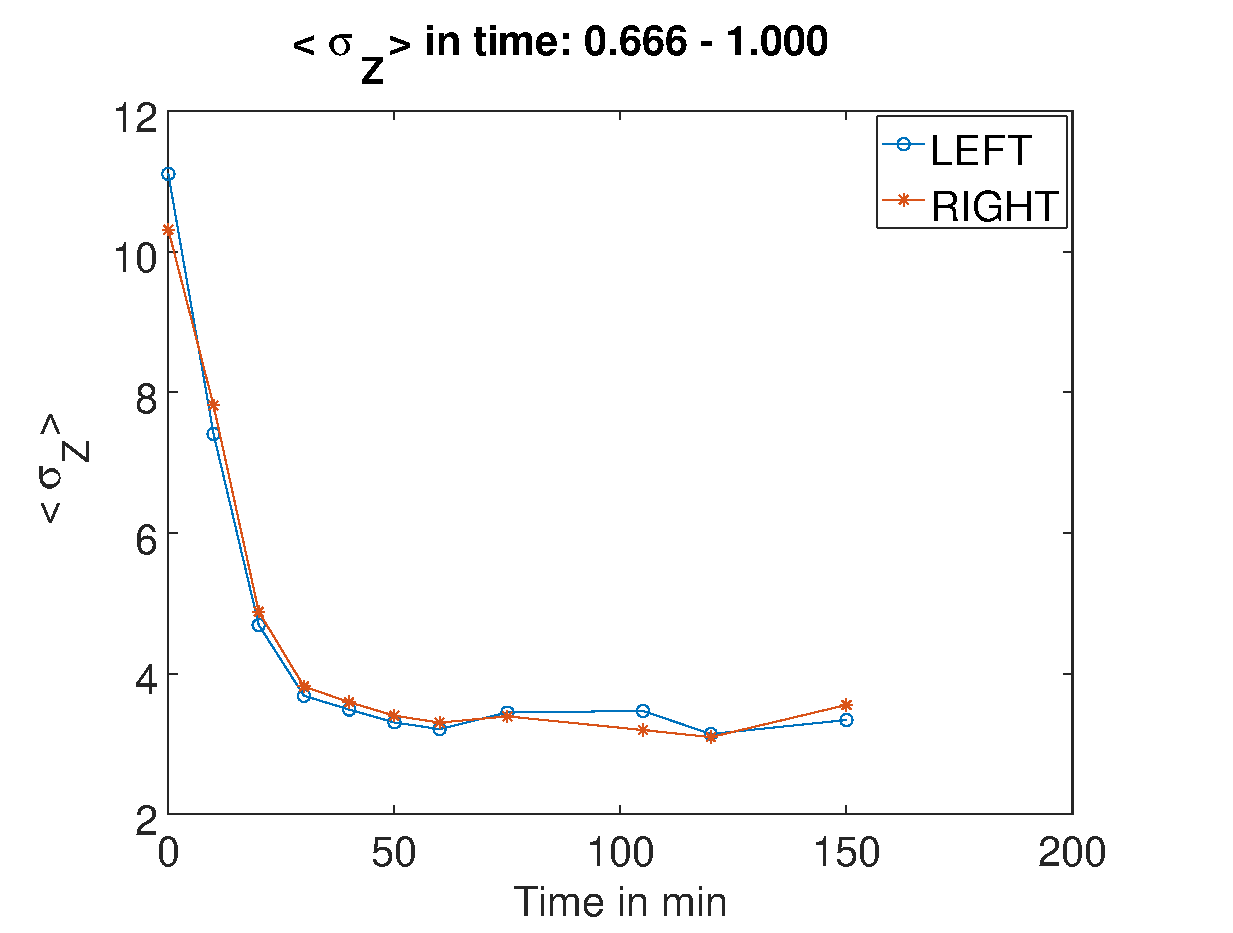
\includegraphics[width=\textwidth]{std-bandz.eps}
	\caption{$\bar{\sigma}_Z$ over time.}
        \label{fig:stdzink}
    \end{subfigure}
    
\caption{Numerical results for the ink drying test.}\label{fig:numerical}
\end{figure}

As can be seen, when we analysed the index over the complete frequency band (Fig.~\ref{fig:allink}),
the two different levels of illumination provided different results, high on the left 
side of Fig.~\ref{fig:regions} and low on the right. This 
indicates a positive influence of the level of illumination on the index.
On the other hand, %Figs~\ref{fig:stdxink}, 
\ref{fig:stdyink} and \ref{fig:stdzink}
show how the index under different levels of illumination are similar when compared at the same frequency component,
with the greatest similarity in the frequency band between $\frac{2}{3}\frac{F_s}{2}$ and $\frac{F_s}{2}$ Hz.

It is important to stress that in the ink drying test, the information 
from the dynamic laser speckle is linked to the high frequencies in the beginning of 
the drying process but with speckle signals with low frequencies at the end, with a gradual transition
until reaching the lowest 
level of the signal in the ink drying test, leaving
%level of the signal, with 
only the speckle signal of the glass plate.
In Fig.~\ref{fig:numerical} ($c-d$) one can see that after 50 minutes there is a 
transition of state with the stabilization of the DLSI. Thus, after this point, 
one has only the glass plate speckle signal influencing the DLSI.

This indicates that the comparisons of the dependence of the index on the level of illumination
should only be made during the first few minutes because after that, we will be using the high contribution of 
the unwanted signals (noise) as the outcome.

\subsection{Numerical results of steady paper under laser light} 
\label{subsec:numericalpaper}

%light intensity with increasing the radius.

Even though the activity level of a piece of paper 
is considered as noise in the context of other tests, which are taking place over it, 
with
%and although it is 
a process of greater activity with variations in time and space;
for the speckle signal analysis of a piece of paper 
we consider it to be approximately homogeneous in its characteristics over time and space,
so as to determine the effect on the dynamic speckle analysis of varying only one parameter, the intensity of the illumination. 

Fig.~\ref{fig:papelstd} presents the result of processing the data of the dynamic laser speckle phenomenon gathered from a steady
 piece of paper,
considering the homogeneous behaviour of the speckle signal and using the standard deviation $\sigma$ 
as a dynamic laser speckle index (DLSI).
Fig.~\ref{fig:papelall} represents the $\sigma_T$ matrix with the complete frequency band, while Fig.~\ref{fig:papelstd_stdx}
represents the $\sigma_X$ matrix with the frequency band between $0$ and $\frac{1}{3}\frac{F_s}{2}$\ Hz.
Fig.~\ref{fig:papelstd_stdy} represents the $\sigma_Y$ matrix with the frequency band between 
$\frac{1}{3}\frac{F_s}{2}$ and $\frac{2}{3}\frac{F_s}{2}$ Hz, and Fig.~\ref{fig:papelstd_stdz} 
represents the $\sigma_Z$ matrix with the frequency band between $\frac{2}{3}\frac{F_s}{2}$ and $\frac{F_s}{2}$ Hz.
\begin{figure}[h!]
    \centering
    \begin{subfigure}[b]{0.485\textwidth}
        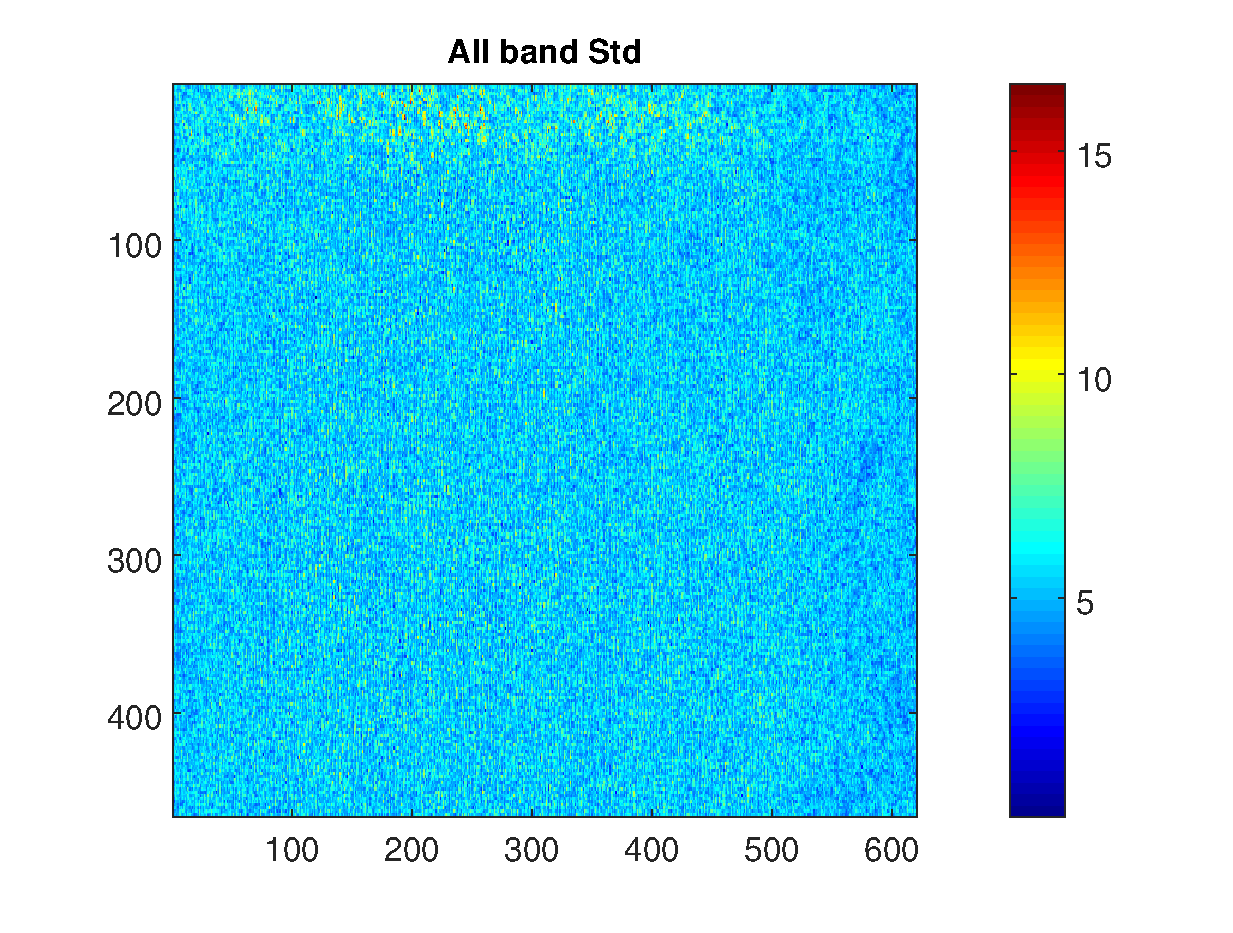
\includegraphics[width=\textwidth]{stdall.eps}
	\caption{$\sigma_T$ matrix over the complete frequency band.}
        \label{fig:papelall}
    \end{subfigure}
    ~
    \begin{subfigure}[b]{0.465\textwidth}
        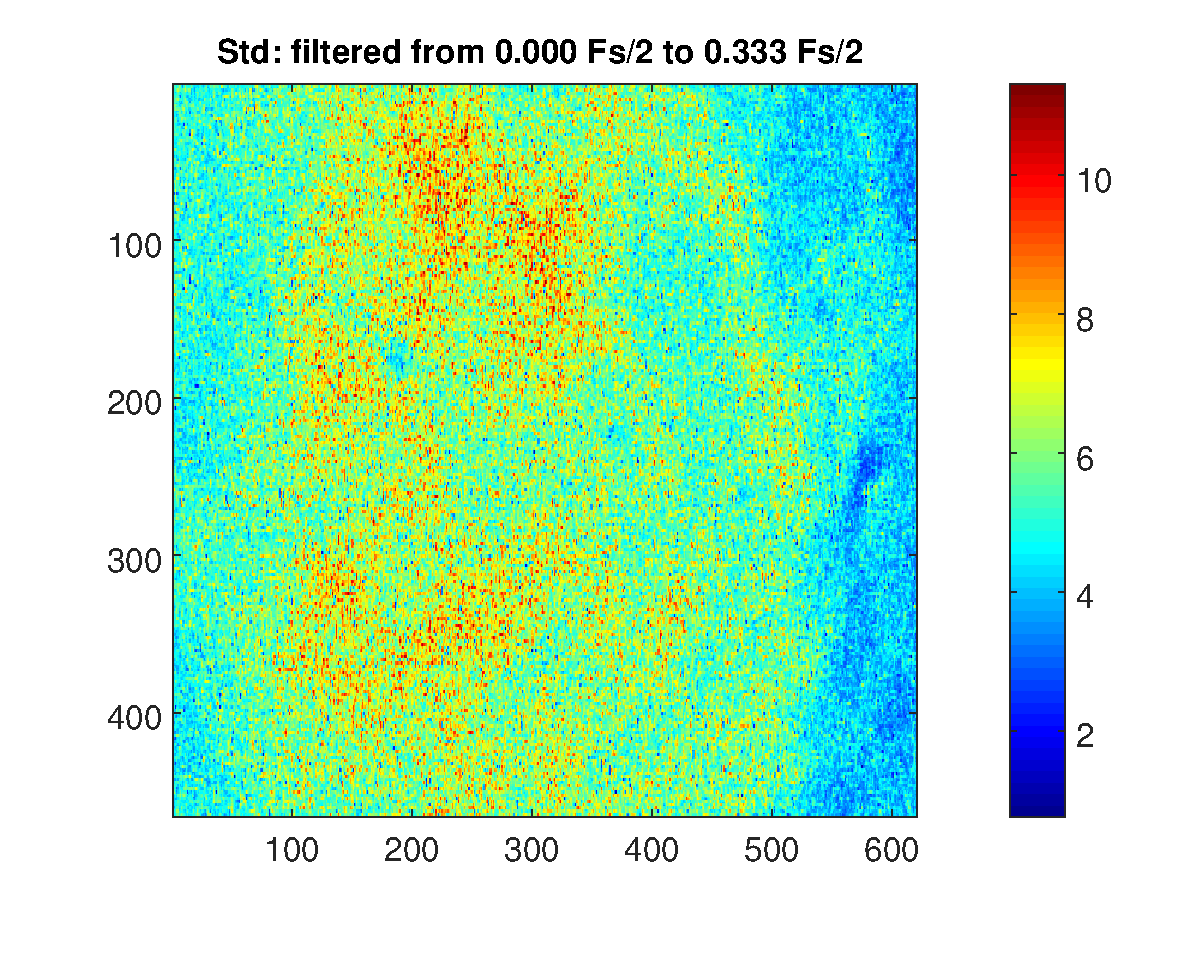
\includegraphics[width=\textwidth]{stdx.eps}
	\caption{$\sigma_X$ matrix over the lower third of the frequency band.}
        \label{fig:papelstd_stdx}
    \end{subfigure}
    ~\\ 
    \begin{subfigure}[b]{0.475\textwidth}
        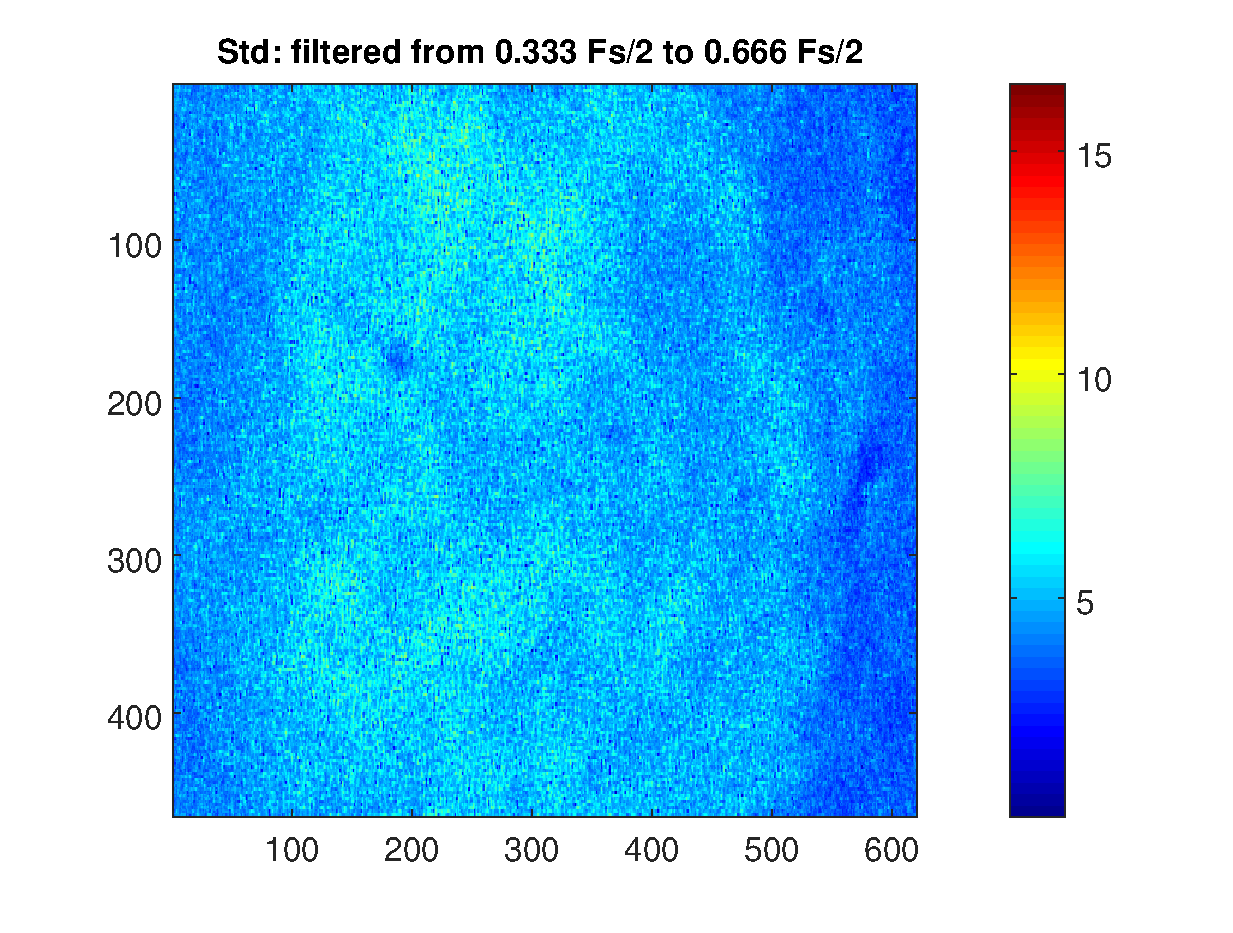
\includegraphics[width=\textwidth]{stdy.eps}
	\caption{$\sigma_Y$ matrix over the middle third of the frequency band.}
        \label{fig:papelstd_stdy}
    \end{subfigure}
  ~
    \begin{subfigure}[b]{0.475\textwidth}
        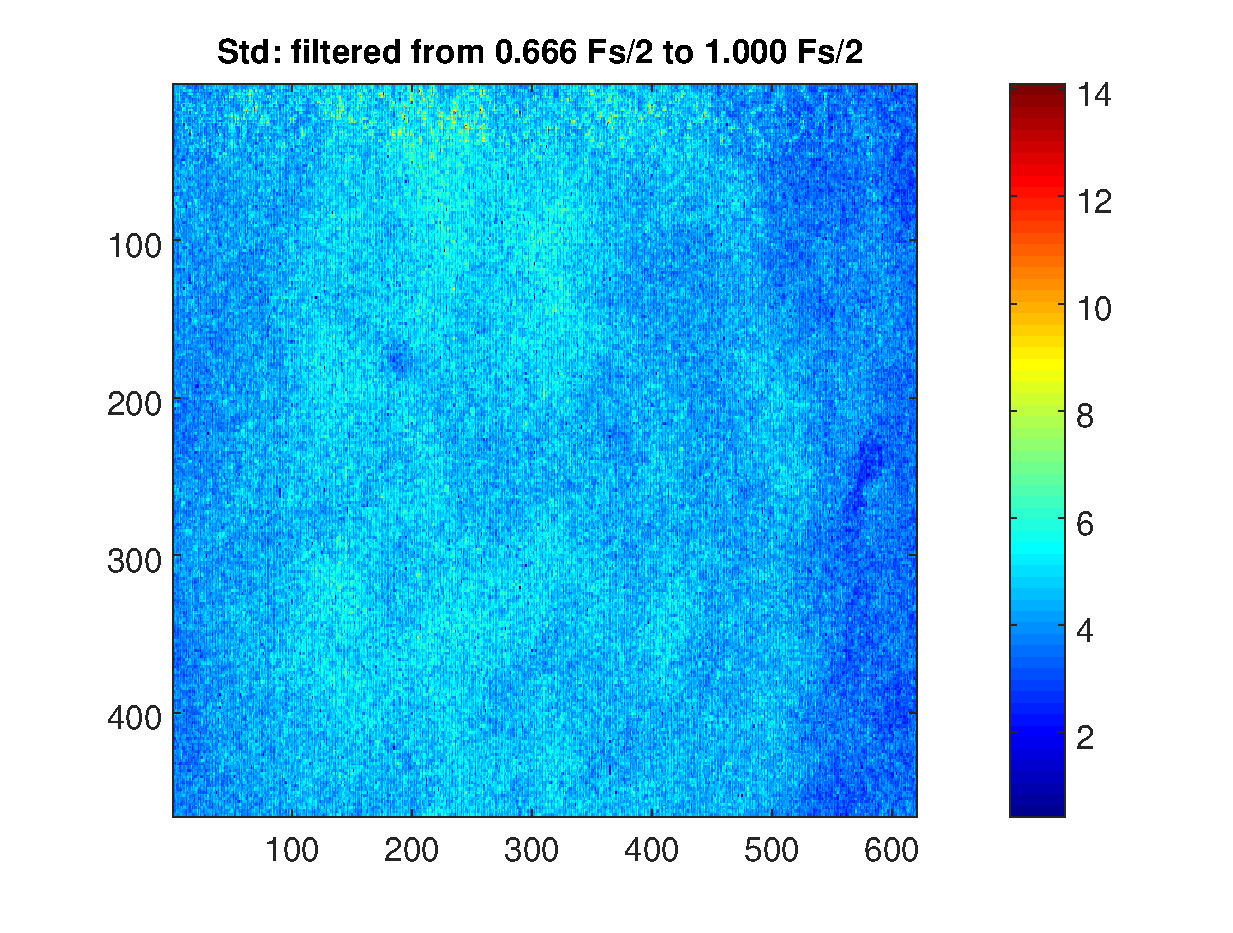
\includegraphics[width=\textwidth]{stdz.eps}
	\caption{$\sigma_Z$ matrix over the upper third of the frequency band.}
        \label{fig:papelstd_stdz}
    \end{subfigure}
    
    \caption{Temporal speckle deviation matrix of a piece of paper.}
    \label{fig:papelstd}
\end{figure}


Fig.~\ref{fig:papelilllevel} presents the relation between the average value of $\sigma_p$,
in the $\sigma$ matrix, with the value of $\mu_p$ (the mean value representing the observable level of illumination) of the $\mu$ matrix, 
in the complete frequency band, the value $\mu_p$
is related to the level of the laser illumination of the surface of the sample \cite{Nothdurft:05}
and its colour. Thus, when we choose $\mu_p$  as reference
in a homogeneous sample,
we are choosing indirectly the observable level of illumination in the surface.
Therefore, Fig.~\ref{fig:papelilllevel} shows the variables $\sigma_p$, $e_p$ and $L_p$ as functions
of  $\mu_p$, for the case of the complete frequency band (\ref{fig:illlevel_all}), 
the lower third of the frequency band (\ref{fig:illlevel_stdx}),
the middle third of the frequency band (\ref{fig:illlevel_stdy}) 
and the upper third of the frequency band (\ref{fig:illlevel_stdz}).
It is important to note that $e_p$ was reinterpreted and plotted as a relation of $\sigma_p$, this means  $100 \frac{e_p}{\sigma_p}\%$,
and $L_p$ is the histogram of the values in the temporal speckle mean matrix.
Given that the mean value is zero for any frequency band without the zero frequency,
the figures show the values of $L_p$ for the complete frequency band, 
with the objective of having a reference for the level of illumination and the number of pixels involved in the analysis.

\begin{figure}[h!]
    \centering
    \begin{subfigure}[b]{0.475\textwidth}
        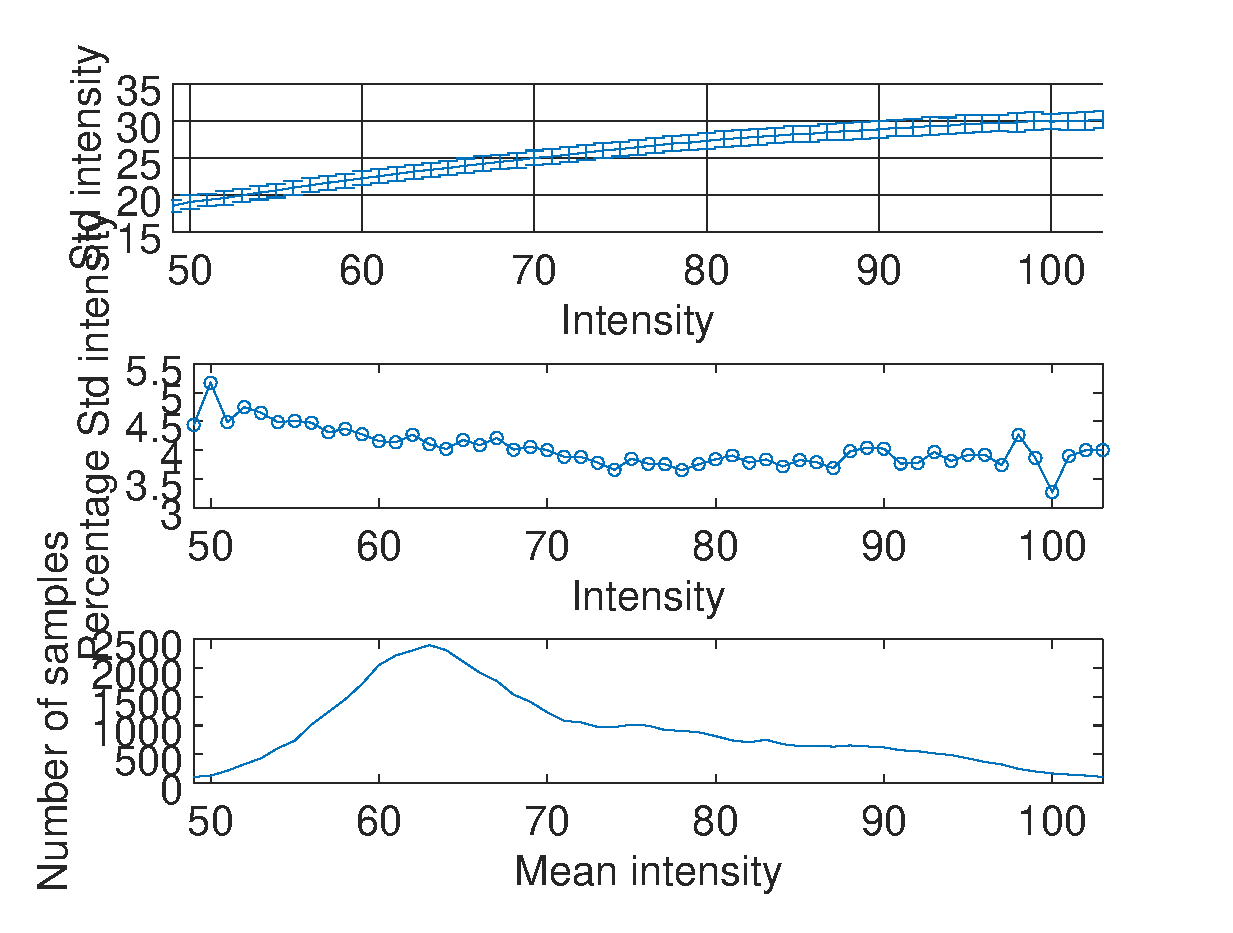
\includegraphics[width=\textwidth]{stdall_curve.eps}
	\caption{Analysis in the complete frequency band.}
        \label{fig:illlevel_all}
    \end{subfigure}
    ~
    \begin{subfigure}[b]{0.475\textwidth}
        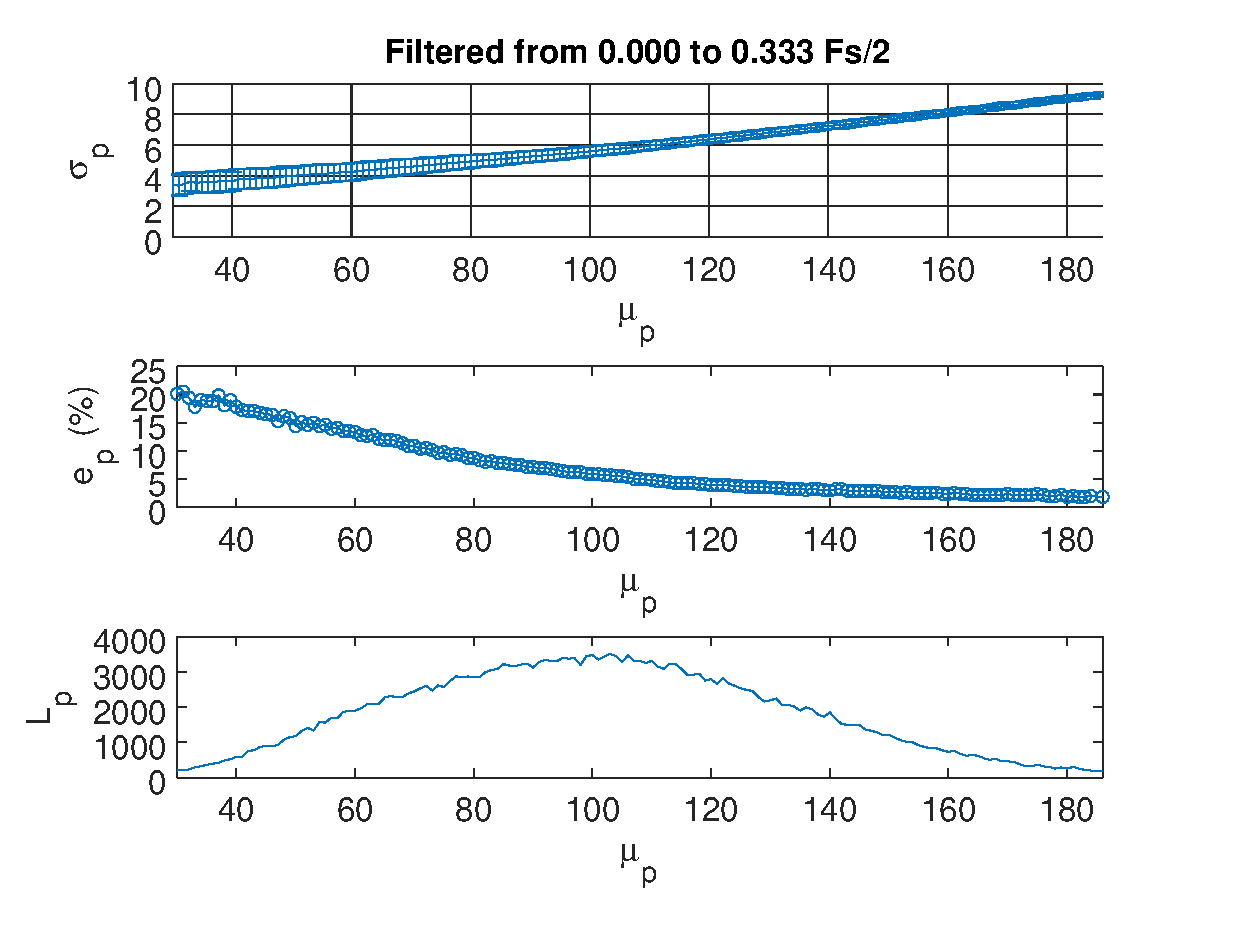
\includegraphics[width=\textwidth]{stdx_curve.eps}
	\caption{Analysis in the lower third of the frequency band.}
        \label{fig:illlevel_stdx}
    \end{subfigure}
    ~\\ 
    \begin{subfigure}[b]{0.475\textwidth}
        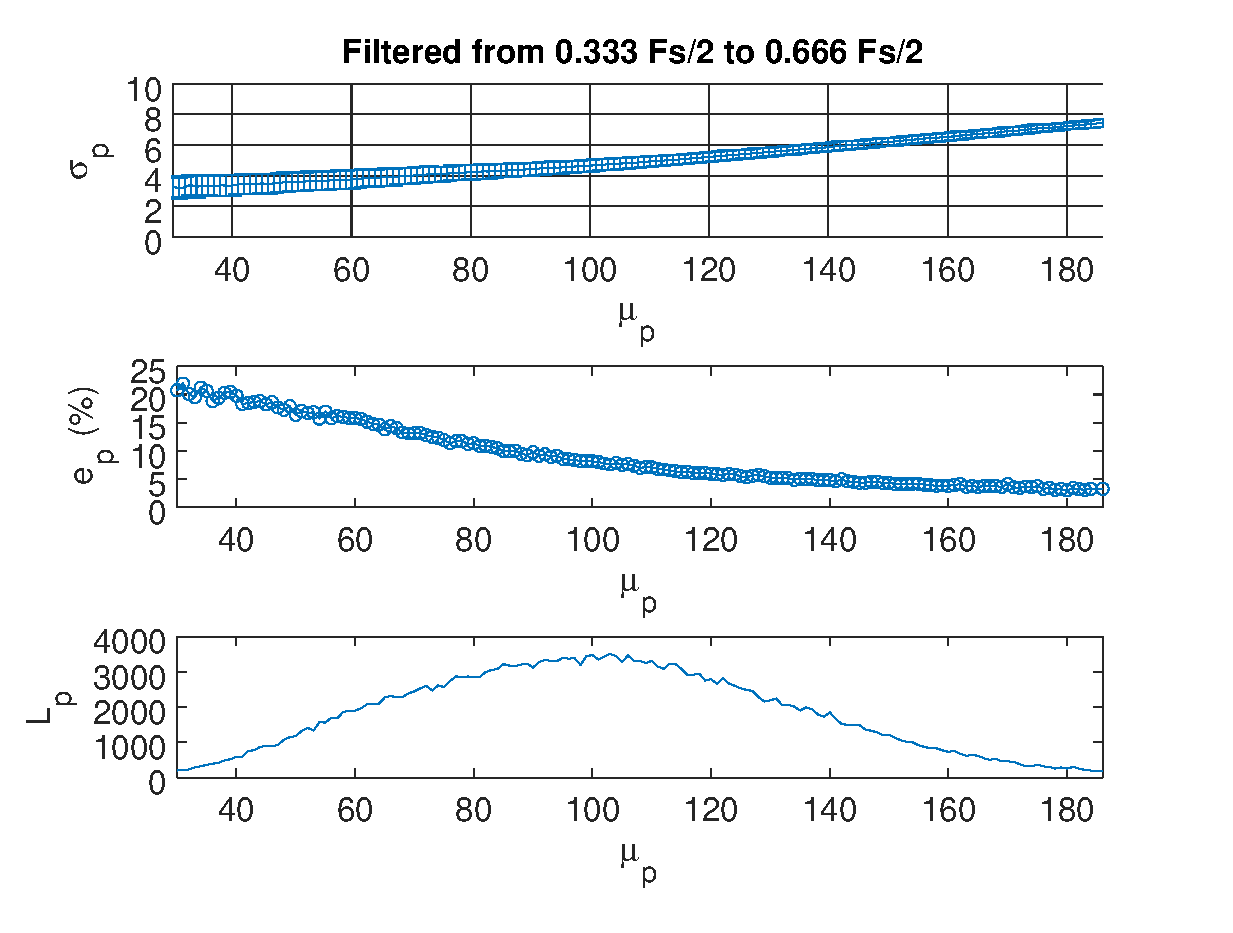
\includegraphics[width=\textwidth]{stdy_curve.eps}
	\caption{Analysis in the middle third of the frequency band.}
        \label{fig:illlevel_stdy}
    \end{subfigure}
  ~
    \begin{subfigure}[b]{0.475\textwidth}
        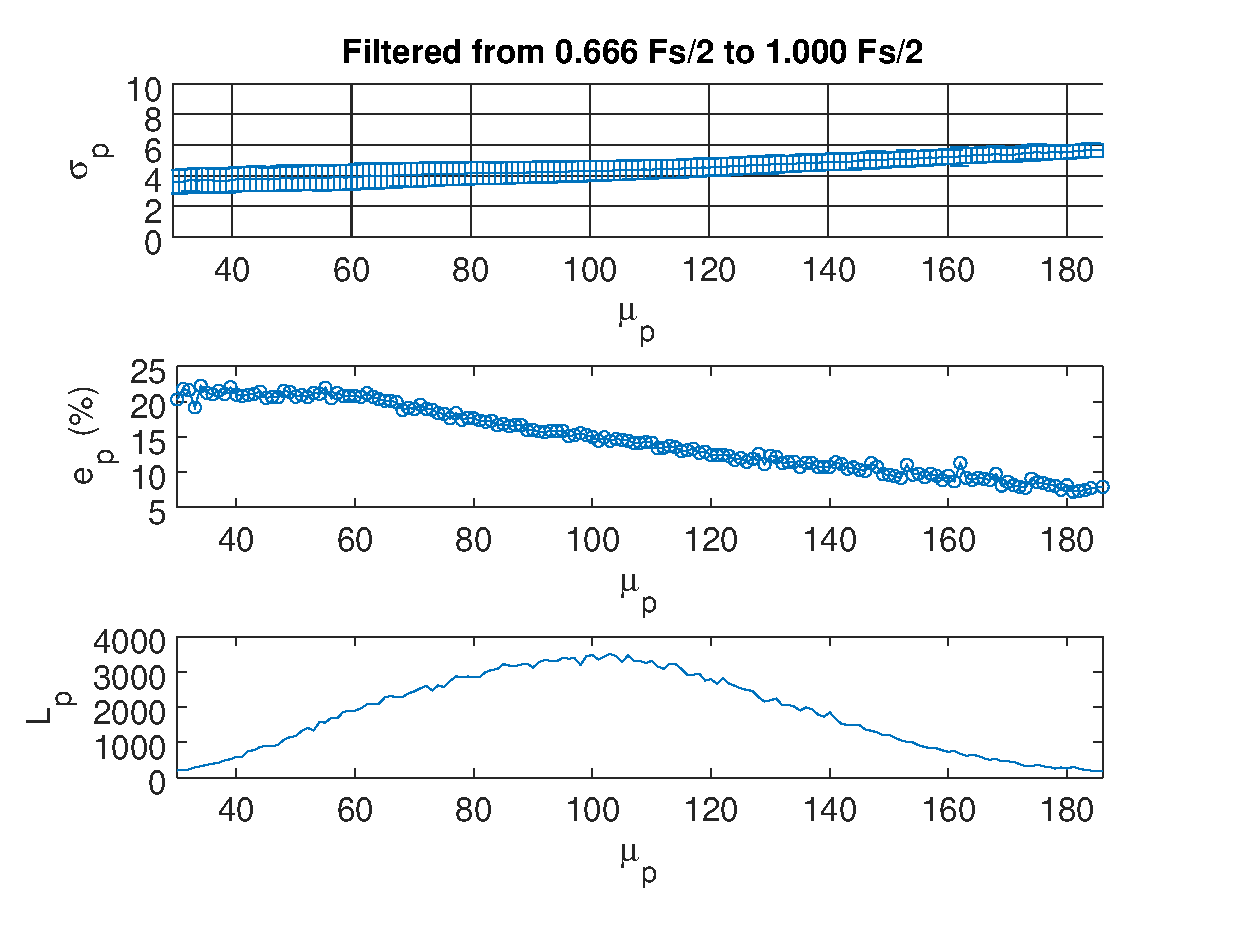
\includegraphics[width=\textwidth]{stdz_curve.eps}
	\caption{Analysis in the upper third of the frequency band.}
        \label{fig:illlevel_stdz}
    \end{subfigure}
    
    \caption{Relation between the standard deviation and the level of illumination for steady paper under laser illumination.}
    \label{fig:papelilllevel}
\end{figure}

In Fig.~\ref{fig:illlevel_all}, we can see the absence of a tendency in the DLSI ($\sigma$) 
with respect to the intensity ($\mu$), 
i.e. with an increase of $\mu$, the standard deviation ($\sigma$) neither increases nor decreases.
However, around that constant there is a uncertainty of $\sigma$ for each value of $\mu$, which creates an uncertainty in the outcome, 
and is expressed by the error $e$.
Fig.~\ref{fig:illlevel_all} represents the outcome from the data without filtering, thus with all frequencies.
The data are the speckle signals present in a material with low activity, 
because the sample is a steady paper approximately homogeneous over time and space.
Nevertheless, when we filter the signal (images in time), 
we observe a change in $\sigma$ with respect to the frequency range, 
revealing the dependence of the DLSI on the level of illumination and its relation with the frequency.
In Fig.~\ref{fig:illlevel_stdx}, corresponding to the lower third of the frequency band, 
there is a tendency of $\sigma$ with respect to the level of illumination.
The DLSI changes its value with  changes in the level of illumination $\mu_p$:
at low levels of illumination we have the highest error, 
but the error tends to zero when the level of illumination ($\mu_p$) increases in some areas of the sample.
The same happens in the middle of the frequency band, 
but much less in the upper third of the frequency band, 
meaning that in the highest frequencies there is less influence of the level of illumination on $\sigma$.
Since the 
temporal speckle deviation index
%$\sigma$ DLSI 
does not filter the signal \cite{RIVERA2017144}, 
this phenomenon must be taken into consideration during the use of this DLSI, 
and how this can compromise the outcome by the influence of the illumination of the sample on the results.
Other dynamic laser speckle indices may offer other options to avoid this influence,
for example, using the Absolute Value of the Differences DLSI and its variations \cite{BSLTLBOOK}.

\subsection{The Fujii index in the ink drying test} 
\label{subsec:vsfujii}

Fig.~\ref{fig:fujiiallink} shows the behaviour of the mean value of the Fujii matrix
defined in Eq.~\ref{eq:contFujii2}.
Figs~\ref{fig:fujiixink}, \ref{fig:fujiiyink} and \ref{fig:fujiizink},
show the behaviour of the mean value of the Fujii matrix defined in Eq.~\ref{eq:contFujii3},
for the frequency bands X, Y and Z, respectively. All cases treat the ink drying test.
\begin{figure}[!h]
    \centering
    \begin{subfigure}[b]{0.475\textwidth}
        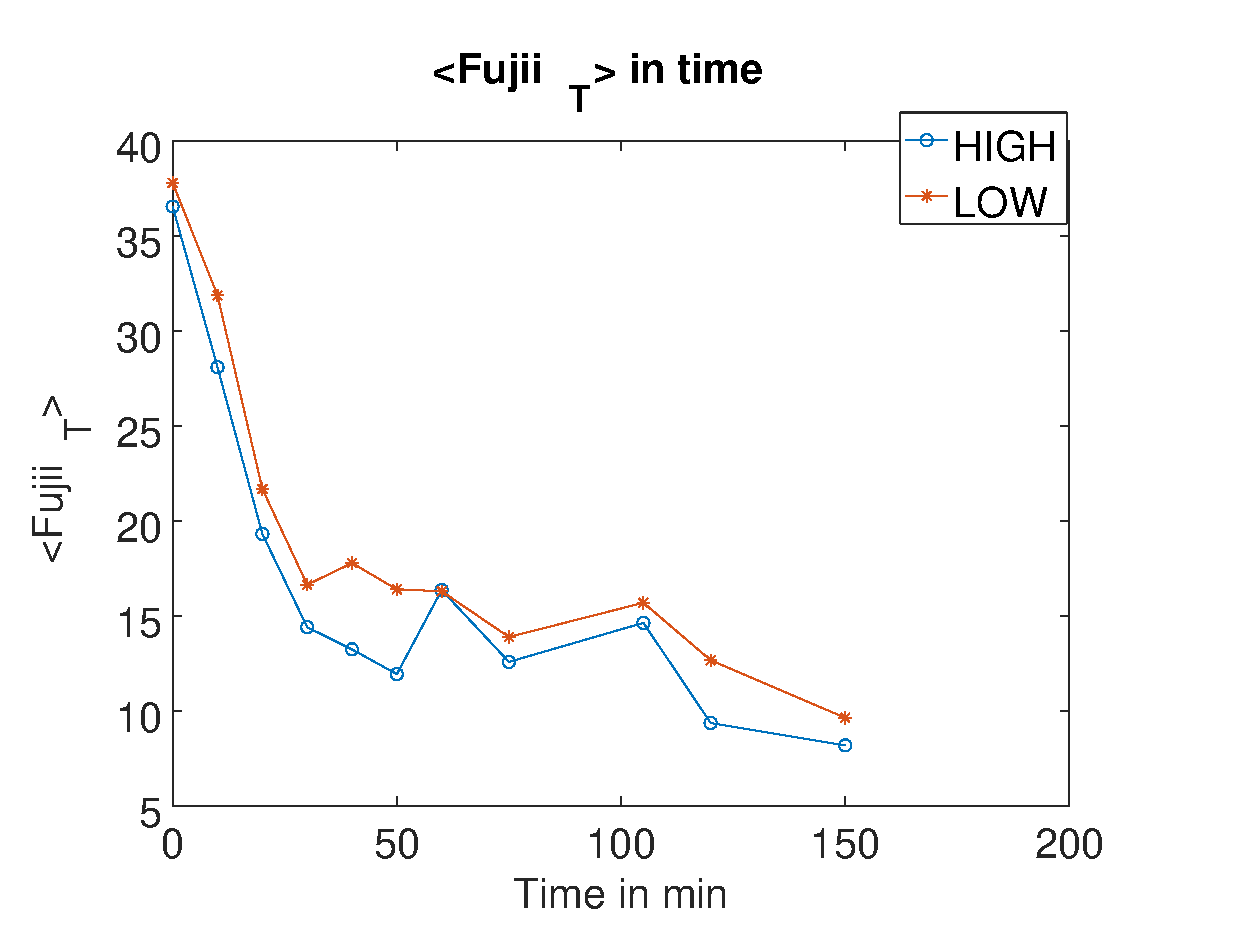
\includegraphics[width=\textwidth]{fujii-all.eps}
	\caption{Fujii value in the complete band.}
        \label{fig:fujiiallink}
    \end{subfigure}
    ~
    \begin{subfigure}[b]{0.475\textwidth}
        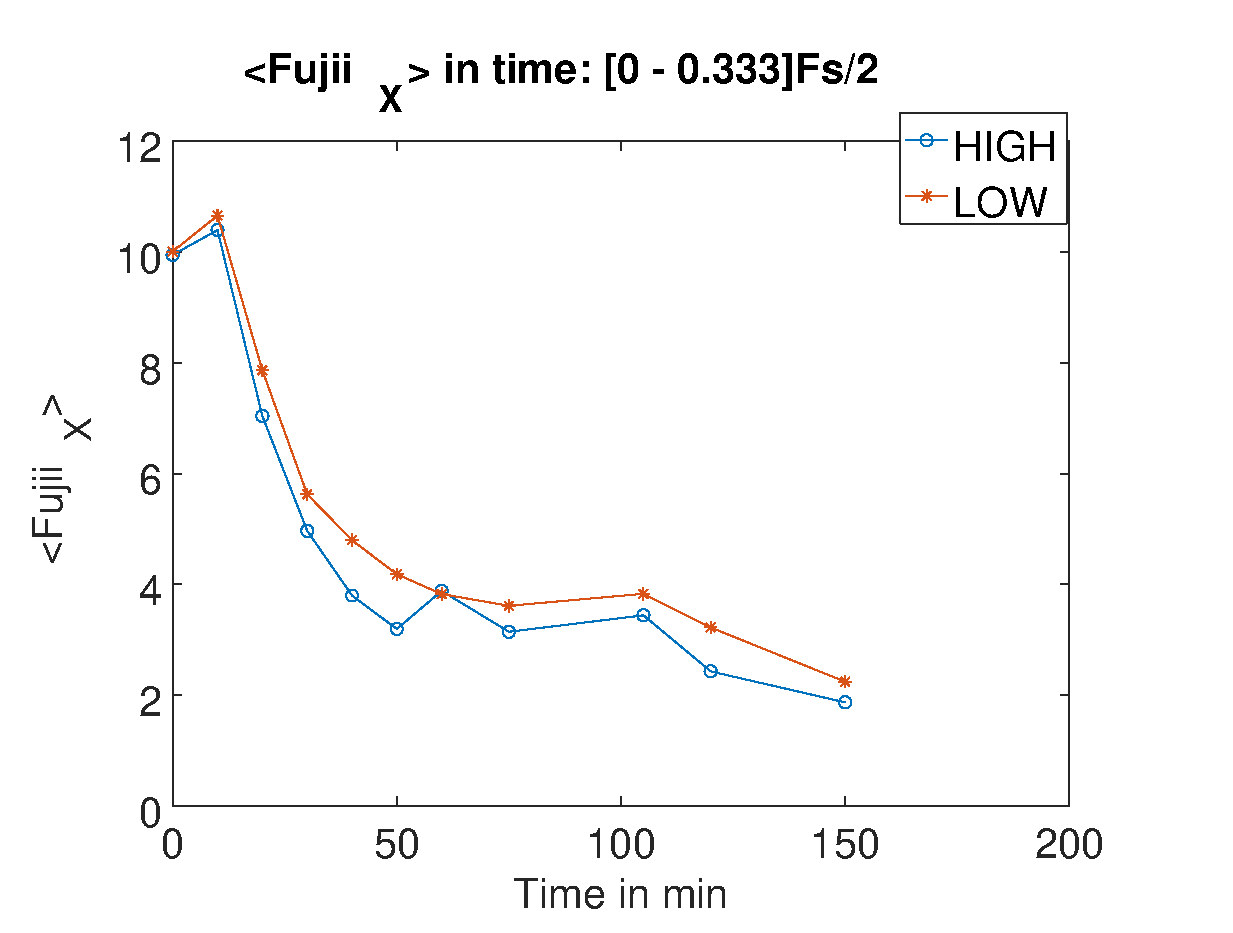
\includegraphics[width=\textwidth]{fujii-bandx.eps}
	\caption{Fujii value in the X band.}
        \label{fig:fujiixink}
    \end{subfigure}
    ~\\ 
    \begin{subfigure}[b]{0.475\textwidth}
        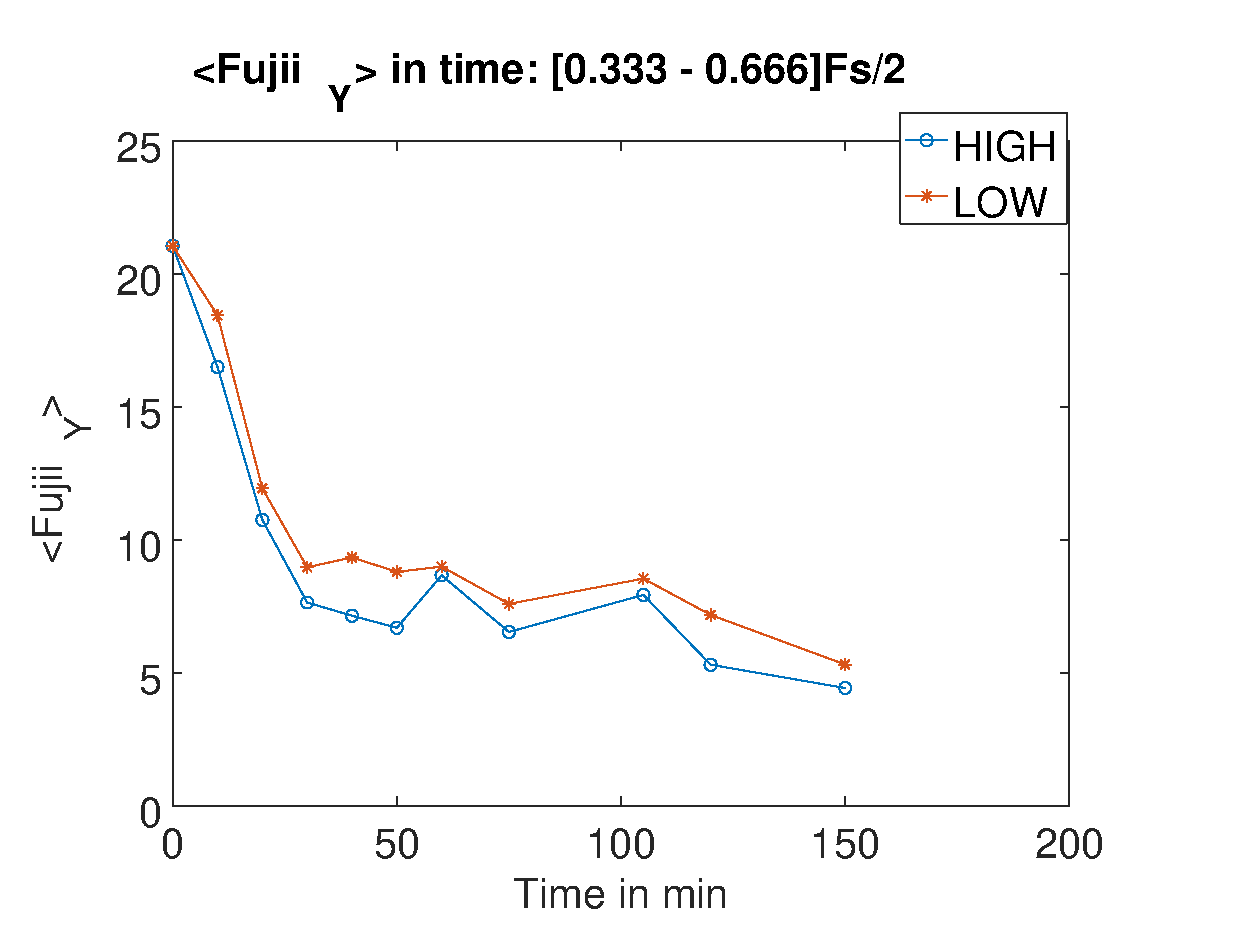
\includegraphics[width=\textwidth]{fujii-bandy.eps}
	\caption{Fujii value in the Y band.}
        \label{fig:fujiiyink}
    \end{subfigure}
  ~
    \begin{subfigure}[b]{0.475\textwidth}
        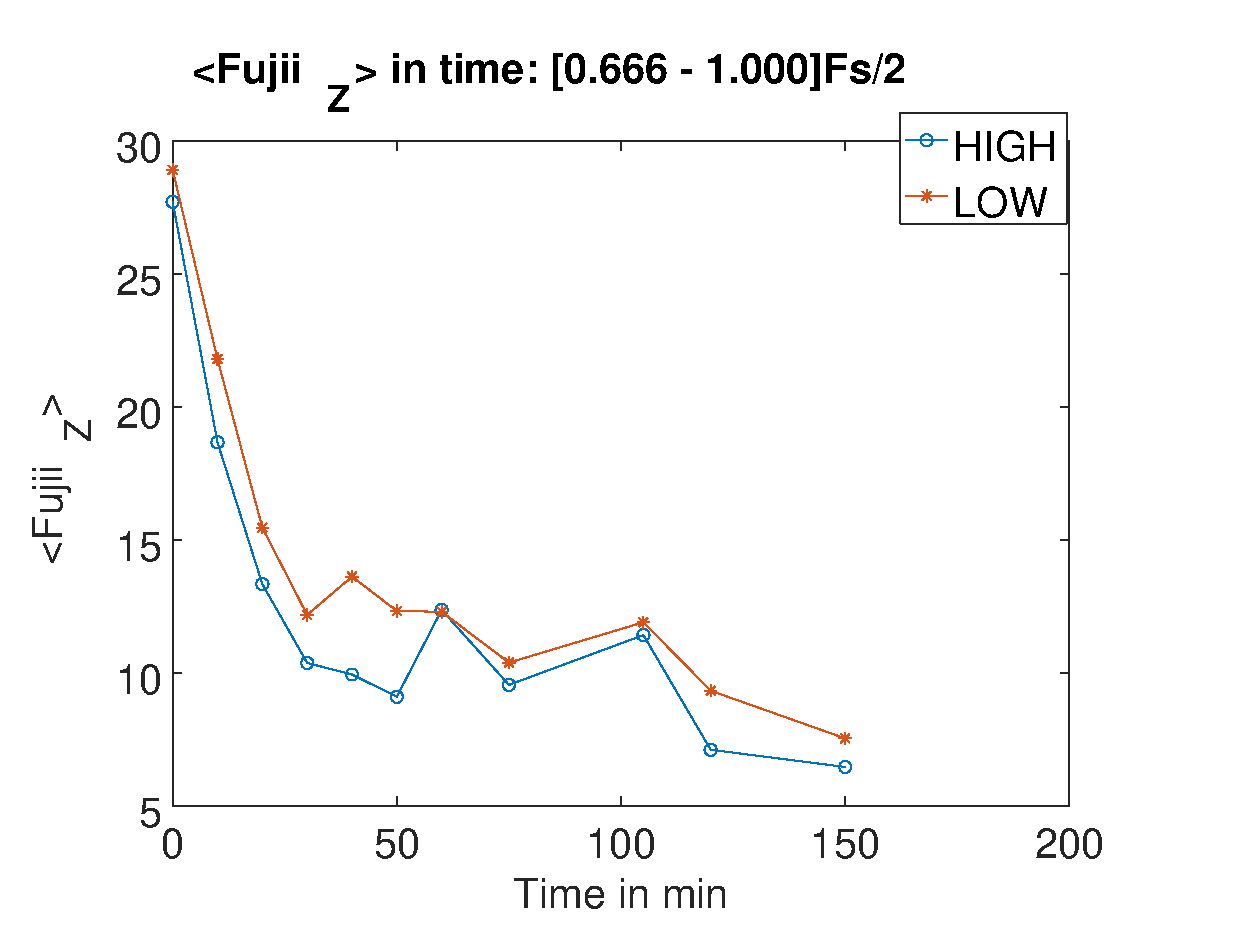
\includegraphics[width=\textwidth]{fujii-bandz.eps}
	\caption{Fujii value in the Z band.}
        \label{fig:fujiizink}
    \end{subfigure}
    
\caption{Numerical results for the ink drying test using the Fujii index.}
\label{fig:numericalvsfujii}
\end{figure}

As can be seen in all the images, the curves with greater or lesser  illumination levels are close,
but there is no advantage in separating the signals by bands.
This can be explained if we analyse how the index synthesizes its value and we compare it with the images.
First, the Fujii index makes a high pass filtering:
this is evident if we look at the maximum values of the curves,
which are greater in the Z (high frequencies) band and rapidly decrease in the Y and X (low frequencies) bands.
Second, the index undergoes a normalization, in the denominator of Eq.~\ref{eq:contFujii2},
with the intention of reducing the dependence of the index on the level of illumination of the sample,
not to mention that this normalization, in the case of a frequency band analysis, is done with the unfiltered signal data.

\section{Final comments} 

Using the results shown in Figs~\ref{fig:numerical} and \ref{fig:papelilllevel},
we can theorize that 
the difference between index values, of a phenomenom to given time,
%the dynamic range between the samples with greater and  lesser values, 
in  the temporal speckle deviation index,
are greater in speckle signals with low frequency components, 
and  smaller in speckle signals with high frequency components;
thus, we can observe that the effect of the level of illumination on 
the variability of the temporal speckle deviation index decreases with the frequency.
This hypothesis is supported by other publications with similar results \cite{Nothdurft:05},
where the temporal speckle mean matrix shows information about the surface of the sample and the ``laser illumination level'', 
and the temporal speckle deviation matrix shows information of the material inside at 
different levels and ``in less proportion the information of the laser illumination level''.
Given that the mean value collects information of the zero frequency component in the speckle signal, 
and the standard deviation  collects information of the non-zero frequency components,
we can make a parallel
with the results obtained in the present paper,
which indicates that, to a given time, the speckle signals with high frequency components
 are less affected in their index values by the variation of the intensity of the laser illumination.
By analysing the Fujii index, 
we also stress that generalizations cannot be made for all speckle indices.
In this paper we mainly used the standard deviation, because its calculation is directly linked to the value, 
or amplitude, of the root mean square of the signals.
In contrast, the Fujii index makes a previous filtering (subtract a sample from the previous one) 
and a non-linear scaling with respect to the light intensity (divide by the average intensity of the two consecutive samples), 
which hinders a fair interpretation of its behaviour for different frequency bands.

\section{Conclusion} 

In the ink drying test, 
we analysed a process that changes its behaviour over time,
and have seen the effect produced on  the speckle light intensity, 
and consequently on the standard deviation index, 
produced by the separation of the signals into different frequency bands.
On the other hand, in the test using a piece of paper, 
we took into consideration the fact that no material is completely inert and, consequently, 
the observed signal  in the  dynamic speckle analysis has more than just noise.

By the analysis of a piece of paper, as shown in Figs~\ref{fig:illlevel_stdx}, \ref{fig:illlevel_stdy} and \ref{fig:illlevel_stdz};
we can see that the greater the observable laser illumination level $\mu_p$, 
the greater will be the $\sigma_p$ index of each pixel analysed. 
However, this increase depends on the frequency band in the speckle signal  analysed;
for example, in Fig.~\ref{fig:illlevel_stdz},
with high frequency components, the relation between $\mu_p$ and $\sigma_p$ is almost a horizontal line, 
which means that a variation of $\mu_p$ does not affect significantly the $\sigma_p$ index.
This is reaffirmed by the analysis of the ink drying test, 
seen in Figs~\ref{fig:stdxink}, \ref{fig:stdyink} and \ref{fig:stdzink},
where the curves of regions with high and low luminosity are compared in different frequency bands:
here, the high frequency band  (Fig.~\ref{fig:stdzink}) 
is the one that produces very similar indices, despite the difference in the level of illumination.

Thus, this paper compared the values of the temporal 
speckle deviation index for three different frequency bands of the speckle signal and 
different levels of illumination in a dynamic laser speckle analysis.
The results showed that the influence of the observable level of illumination on the DLSI, 
like the temporal speckle deviation index, 
decreases with the use of signals with high frequency components.

\section{Acknowledgment}
We wish to acknowledge the partial financial support for this study provided by the CAPES
scholarship
PNPD Program, FAPEMIG and CNPQ.

\section{Bibliography}
\bibliography{report}
\bibliographystyle{spiebib}
\end{document} 

